%\RequirePackage{lineno}
%\documentclass[aps,prc,preprint,superscriptaddress,showpacs,showkeys]{revtex4-1} %%PRC class
\documentclass[12pt,a4paper,final]{iopart} %% JPG class
\newcommand{\Jpsi}{J/\psi}
\newcommand{\pT}{p_{T}}
\newcommand{\sNN}{\sqrt{s_{_{NN}}}}
\newcommand{\raa}{R_{AA}}
\newcommand{\ccbar}{\rm{c\overline{c}}}
\newcommand{\bbbar}{\rm{b\overline{b}}}
\newcommand{\npart}{N_{\rm part}}

%\usepackage{graphicx}
%%\usepackage{cite}
%\usepackage[usenames,dvipsnames,svgnames,table]{xcolor}
%%\usepackage{amsmath}
%%\usepackage{mathtools}

\usepackage{verbatim}
\usepackage{graphicx}
\usepackage[usenames,dvipsnames,svgnames,table]{xcolor}
\usepackage[breaklinks=true,colorlinks=true,linkcolor=blue,urlcolor=blue,citecolor=blue]{hyperref}
\usepackage{rotating}
\usepackage{graphicx}% Include  files
\usepackage{dcolumn}% Align table columns on decimal point
\usepackage{bm}% bold math
\usepackage{epsfig}
\usepackage{hyperref}
\usepackage{ulem}
\usepackage{appendix}
\usepackage{iopams}
%\usepackage{mwe}
\usepackage{subfig}
\expandafter\let\csname equation*\endcsname\relax
\expandafter\let\csname endequation*\endcsname\relax
\usepackage{amsmath}



\begin{document}

\title[]{Suppression of quarkonia in PbPb collisions at $\sqrt{s_{NN}}$ =  5.02 TeV}
%\linenumbers
\author{Vineet Kumar}
\address{Nuclear Physics Division, Bhabha Atomic Research Center, Mumbai, India}
\ead{Vineet.Kumar@cern.ch}
\author{Prashant Shukla}
\address{Nuclear Physics Division, Bhabha Atomic Research Center, Mumbai, India}
\address{Homi Bhabha National Institute, Anushakti Nagar, Mumbai, India}
%\email{pshukla@barc.gov.in}
\author{Abhijit Bhattacharyya}
\address{Department of Physics, University of Calcutta, 92, A. P. C. Road Kolkata-700009, India}
%\ead{abphy@caluniv.ac.in}


\date{\today}

\begin{abstract}
  
  We study different processes responsible for the modification of quarkonia yields
in the medium produced in PbPb collisions at $\sqrt{s_{NN}}$ =  5.02 TeV.
The quarkonia and heavy flavour cross sections are estimated using the measurements in
pp collisions at LHC energies and shadowing corrections are obtained using the EPS09
parametrizations. A kinetic model is used which incorporates quarkonia suppression
inside the Quark Gluon Plasma (QGP), suppression due to hadronic comovers, and regeneration
from recombination of heavy quark pairs. The quarkonia dissociation cross section due to gluon 
collisions, including both color-electric dipole and color-magnetic dipole transitions,
has been employed. The regeneration rate is obtained using the principle of 
detailed balance. The effect of these processes on the nuclear modification
factors for both $\Jpsi$ and $\Upsilon$ in different ranges of transverse momentum
$\pT$ and rapidity has been studied for PbPb collisions at $\sNN =$ 5.02 TeV. The calculations
are compared with the available results from LHC experiments. Both the suppression
and regeneration due to a QGP are effective in the low and intermediate $\pT$ range.
The large observed suppression of $\Jpsi$ at
$\pT~>$ 10 GeV/$c$ is larger than the suppression expected due to gluon dissociation.

\end{abstract}

\pacs{12.38.Mh, 24.85.+p, 25.75.-q}
%%\keywords{quark-gluon plasma, quarkonia, suppression, regeneration}

\maketitle

%%%%%%%%%%%%%%%%%%%%%%%%%%%%%%%%%%%%%%%%%%%%%%%%%%%%%%%%%%%%%%%%%%%%%%%%%%%%%%%%%%%%%%%%%%%%%%%%%%%%%%%%%%%%%%%%%
\section{Introduction}

Quantum chromodynamics (QCD) predicts that strongly interacting matter undergoes a phase
transition to quark-gluon plasma (QGP), a state in which quarks and gluons move much beyond the
size of hadrons. Heavy-ion collisions at relativistic energies are performed to create and
quantify the properties of QGP~\cite{Busza:2018rrf,Shuryak:2017aol}. Charmonia and bottomonia,
which are bound states of charm-anticharm (c$\bar{\rm c}$) or bottom-antibottom (b$\bar{\rm b}$) quarks,
respectively, are among the most sensitive probes of the characteristics of the QGP~\cite{Brambilla:2010cs}.
%A suppression of their yields in nucleus-nucleus collisions with respect to expectations
%from proton-proton collisions was proposed as a smoking gun signal of QGP
%formation~\cite{Matsui:1986dk,Hashimoto:1986nn}.
These bound states of heavy quarks are formed early in the heavy ion collisions and their
yields are expected to be suppressed in the medium as compared to their yields in pp
collisions ~\cite{Matsui:1986dk,Hashimoto:1986nn}. 
 There have been a large number of studies on this phenomenon both theoretically and 
 experimentally~\cite{Brambilla:2010cs,Schukraft:2013wba,Andronic:2015wma} 
 enriching our understanding on quarkonia as probes of QGP. 
 The J/$\psi$ meson was measured at the SPS, in PbPb and In-In interactions
at the centre-of-mass energy per nucleon pair $\sNN$ = 17.2 GeV~\cite{Alessandro:2004ap,Arnaldi:2007zz},
at RHIC in AuAu interactions at 
$\sNN$ = 200 GeV~\cite{Adare:2011yf,Abelev:2009qaa,Tang:2011kr}, and finally at the LHC,
in PbPb collisions at $\sNN$ = 2.76 and
5.02 TeV~\cite{Aad:2010aa,Chatrchyan:2012np,Khachatryan:2016ypw,Sirunyan:2017isk,ATLAS:2016qpn,Abelev:2013ila,Adam:2016rdg,Acharya:2017tgv}.
The suppression of $\Jpsi$ observed at SPS was termed as 'anomalous' $\Jpsi$
suppression. It was even considered to be a hint of QGP~\cite{Alessandro:2004ap,Arnaldi:2007zz} formation.
Early theoretical calculations predicted $\Jpsi$ suppression due to colour screening
in a deconfined medium which become stronger as the QGP 
temperature increases~\cite{Matsui:1986dk,Digal:2001ue} but the RHIC measurements
at $\sNN$ = 200 GeV showed almost the same amount of suppression, contrary to
expectation~\cite{Brambilla:2010cs,Adare:2011yf}. These observations hint a scenario where,
at higher collision energies, the expected larger suppression is compensated by
$\Jpsi$ regeneration via recombination of two independently produced 
charm quarks~\cite{Andronic:2003zv,Thews:2000rj,Du:2017qkv}. 

The LHC collected first PbPb collision data at $\sNN =$ 2.76 TeV at the end of 2010.
The ATLAS was the first detector to measure 
the ratio of $\Jpsi$ meson with Z$^{0}$ boson hinting a centrality-dependent suppression
of the yield of $\Jpsi$ mesons~\cite{Aad:2010aa}.
 The $\Jpsi$ measurements at high transverse momentum ($p_T>6.5$ GeV/$c$) in PbPb collisions at $\sNN$=2.76 TeV and at
$\sNN$=5.02 TeV were carried out by the CMS experiment~\cite{Chatrchyan:2012np,Khachatryan:2016ypw,Sirunyan:2017isk}.
The nuclear modification factor $R_{AA}$ of these high $p_T$ prompt $\Jpsi$ decreases
with increasing centrality. The $R_{AA}$ shows a slow increase as a function of
$p_T$ after 15 GeV$/c$ and then saturates between a value 0.4 and 0.5 showing that the $\Jpsi$
remains suppressed, even at very high $p_T$, up to $\sim$ 50 GeV/$c$. The ATLAS experiment
also measured $R_{AA}$ of $\Jpsi$ at $\sNN$=5.02 TeV for $\Jpsi$ meson having
transverse momentum above 9.0 GeV$/c$~\cite{ATLAS:2016qpn}. The amount 
of suppression of $\Jpsi$ mesons observed by ATLAS is similar to the suppression
observed by CMS experiment. By comparing these measurements with the STAR
results~\cite{Tang:2011kr} at RHIC, it follows that the suppression of high $p_T~\Jpsi$
increases with collision energy.


  The ALICE experiment measured the nuclear modification factor of $\Jpsi$ mesons 
in the forward rapidity (2.5$<y<$4.0) range at $\sNN$=2.76 and $\sNN$=5.02 
TeV~\cite{Abelev:2013ila,Adam:2016rdg} with $\Jpsi$ transverse momentum starting from
0.3 GeV/$c$.
The ALICE results shows that nuclear modification factor of
low $\pT$ J/$\psi$ ($\pT<$ 12 GeV/$c$) has almost no collision centrality dependence 
except in the most peripheral region where it reaches almost unity.
The $R_{AA}$ of $\Jpsi$ mesons decreases substantially as a function of $\pT$ 
in the ALICE experiment~\cite{Abelev:2013ila,Adam:2016rdg}. The ALICE measurements also
give a hint for an increase of $R_{AA}$ between $\sNN$ = 2.76 and 5.02 TeV in the intermediate
$\pT$ region, 2 $< \pT < $ 6 GeV/$c$. A comparison of 
the ALICE and PHENIX measurements reveal that at LHC, $\Jpsi$ mesons with low $p_T$ are less
suppressed as compared to RHIC. In general the results at LHC experiments when 
compared to the RHIC measurements indicate that the data on $\Jpsi$ production support a 
picture where both suppression and regeneration take place in the QGP, 
the two mechanisms being dominant at high and low $\pT$, respectively~\cite{P.ShuklaforCMS:2014vna,Kumar:2014kfa}.

In addition to $\Jpsi$ mesons the bottomonia states ($\Upsilon$(nS)) are also measured at
the LHC with very good statistical
precision~\cite{Chatrchyan:2011pe,Chatrchyan:2012lxa,Abelev:2014nua,Khachatryan:2016xxp}.
The CMS measurements at $\sNN =$2.76 TeV~\cite{Chatrchyan:2011pe,Chatrchyan:2012lxa} reveal
a clear proof of sequential suppression :  $\Upsilon$(2S) and $\Upsilon$(3S) are 
more suppressed relative to the ground state $\Upsilon$(1S).   The individual $\Upsilon$ states are also found to be suppressed in
the PbPb collisions relative to the production in the pp collisions. The $\Upsilon$ nuclear
modification factor, $R_{AA}$, shows a strong dependence on collision centrality but has
weak dependence on $\Upsilon$ meson $\pT$ and rapidity~\cite{Khachatryan:2016xxp}.
The forward rapidity ($2.5 \leq y^{\Upsilon} \leq 4.0$) measurement of the $\Upsilon$ suppression at 
ALICE~\cite{Abelev:2014nua} is found to be consistent with the midrapidity ($|y^{\Upsilon}|\,\leq 2.4$)
measurement of the $\Upsilon$ suppression at the CMS. 
The CMS and ALICE collaborations have carried out the $\Upsilon\,\, R_{AA}$ measurement
at $\sNN =$ 5.02 TeV with the Run II LHC PbPb
collisions~\cite{Sirunyan:2017lzi,CMS:2017ucd,ALICE:Y5TeV}.
The CMS experiment measured slightly more amount of $\Upsilon$ suppression at
$\sNN =$ 5.02 TeV~\cite{Sirunyan:2017lzi,CMS:2017ucd} than the suppression at
$\sNN =$ 2.76 TeV~\cite{Khachatryan:2016xxp} while the ALICE experiment observed less
suppression at $\sNN =$ 5.02 TeV than that at $\sNN =$ 2.76 TeV 
in the most central PbPb collisions~\cite{Abelev:2014nua,ALICE:Y5TeV}. 

 The field of quarkonia has attracted a large amount of theoretical activities
since the first prediction of $\Jpsi$ suppression in heavy 
ion collisions~\cite{Matsui:1986dk,Hashimoto:1986nn}. 
The color screening
of q$\overline{\rm q}$ potential inside the QGP~\cite{Karsch:1987pv,Abdulsalam:2012bw}
was the first approach to study the suppression of quarkonia
in heavy ion collisions. 
 In a complementary way to this static approach, $\Jpsi$ suppression can also be understood
as a result of dynamical interactions with the surrounding gluons~\cite{Bhanot:1979vb,Chen:2017jje,Kumar:2014kfa}.
One of the ways to calculate the regeneration is to use the principle of detailed balance~\cite{Thews:2000rj}.  
There are other effects also, namely shadowing and comover interaction~\cite{Vogt:2015uba,Ferreiro:2014bia}.
Shadowing arises as the parton distribution functions are modified inside the nucleus. 
A comprehensive framework to explain the experimental data from LHC considering shadowing and 
comover~\cite{Du:2017qkv,Rapp:2017chc} and viscous hydrodynamics~\cite{Krouppa:2015yoa,Krouppa:2017jlg}
has recently been formulated. 

 Some of us have studied the modification of quarkonia yields due to various
processes in AA collisions in a previous work~\cite{Kumar:2014kfa}.
In that work, the gluon dissociation cross section has
been adopted from the calculations of Bhanot and Peskin~\cite{Bhanot:1979vb}
where the gluon dissociation rate has been estimated from operator product expansion
in the Coulomb approximation. Recently, Chen and He have revisited the gluon dissociation
using QCD multipole expansion for various quarkonia in QGP~\cite{Chen:2017jje}.
They reproduced the result of Bhanot and Peskin as the colour-electric 
dipole (E1) transition. They have also calculated the colour magnetic
dipole (M1) transition and found its contribution to be significant
at low energies.
 In this paper, we calculate $\Jpsi$ and $\Upsilon$ evolution
in a kinetic model which includes dissociation by thermal gluons
(both E1 and M1 transitions), modification 
of their yields due to shadowing and due to collisions with comovers.
Regeneration by near thermal heavy quark pairs is also considered in the calculations.
We obtain the nuclear modification factor of quarkonia as a function of the
transverse momentum and centrality of the collision and compare it to the latest
experimental data from LHC at $\sNN =$ 5.02 TeV.






%%%%%%%%%%%%%%%%%%%%%%%%%%%%%%%%%%%%%%%%%%%%%%%%%%%%%%%%%%%%%%%%%%%%%%%%%%%%%%%%%%%%%%%%%
\section{Theoretical formulation}

The theoretical formulation towards the formation and dissociation of quarkonia have already been discussed 
in Ref.~\cite{Kumar:2014kfa}. We use the same formulation here and hence discuss only some important points.


\subsection{Formation and Dissociation}


In the kinetic approach \cite{Thews:2000rj}, the evolution of the quarkonia 
population $N_{Q}$ with the proper time, $\tau$ is given by the kinetic equation

\begin{equation}\label{eqkin}
{dN_{Q} \over d\tau}  =  - \lambda_D  \rho_g N_{Q} + \lambda_F {N_{q \bar{q}}^{2} \over V(\tau)}.
\end{equation}
In the above equation $V(\tau)$ is the spatial volume of the QGP  and $N_{q \bar{q}}$ is
the number of initial heavy quark pairs produced in a event as a function of the centrality
defined by the number of participants $N_{\rm part}$. The $\lambda_{D}$ is the dissociation
rate and the $\lambda_{F}$ is the formation rate. $\rho_g$ is the density of thermal gluons.

 
\begin{figure}
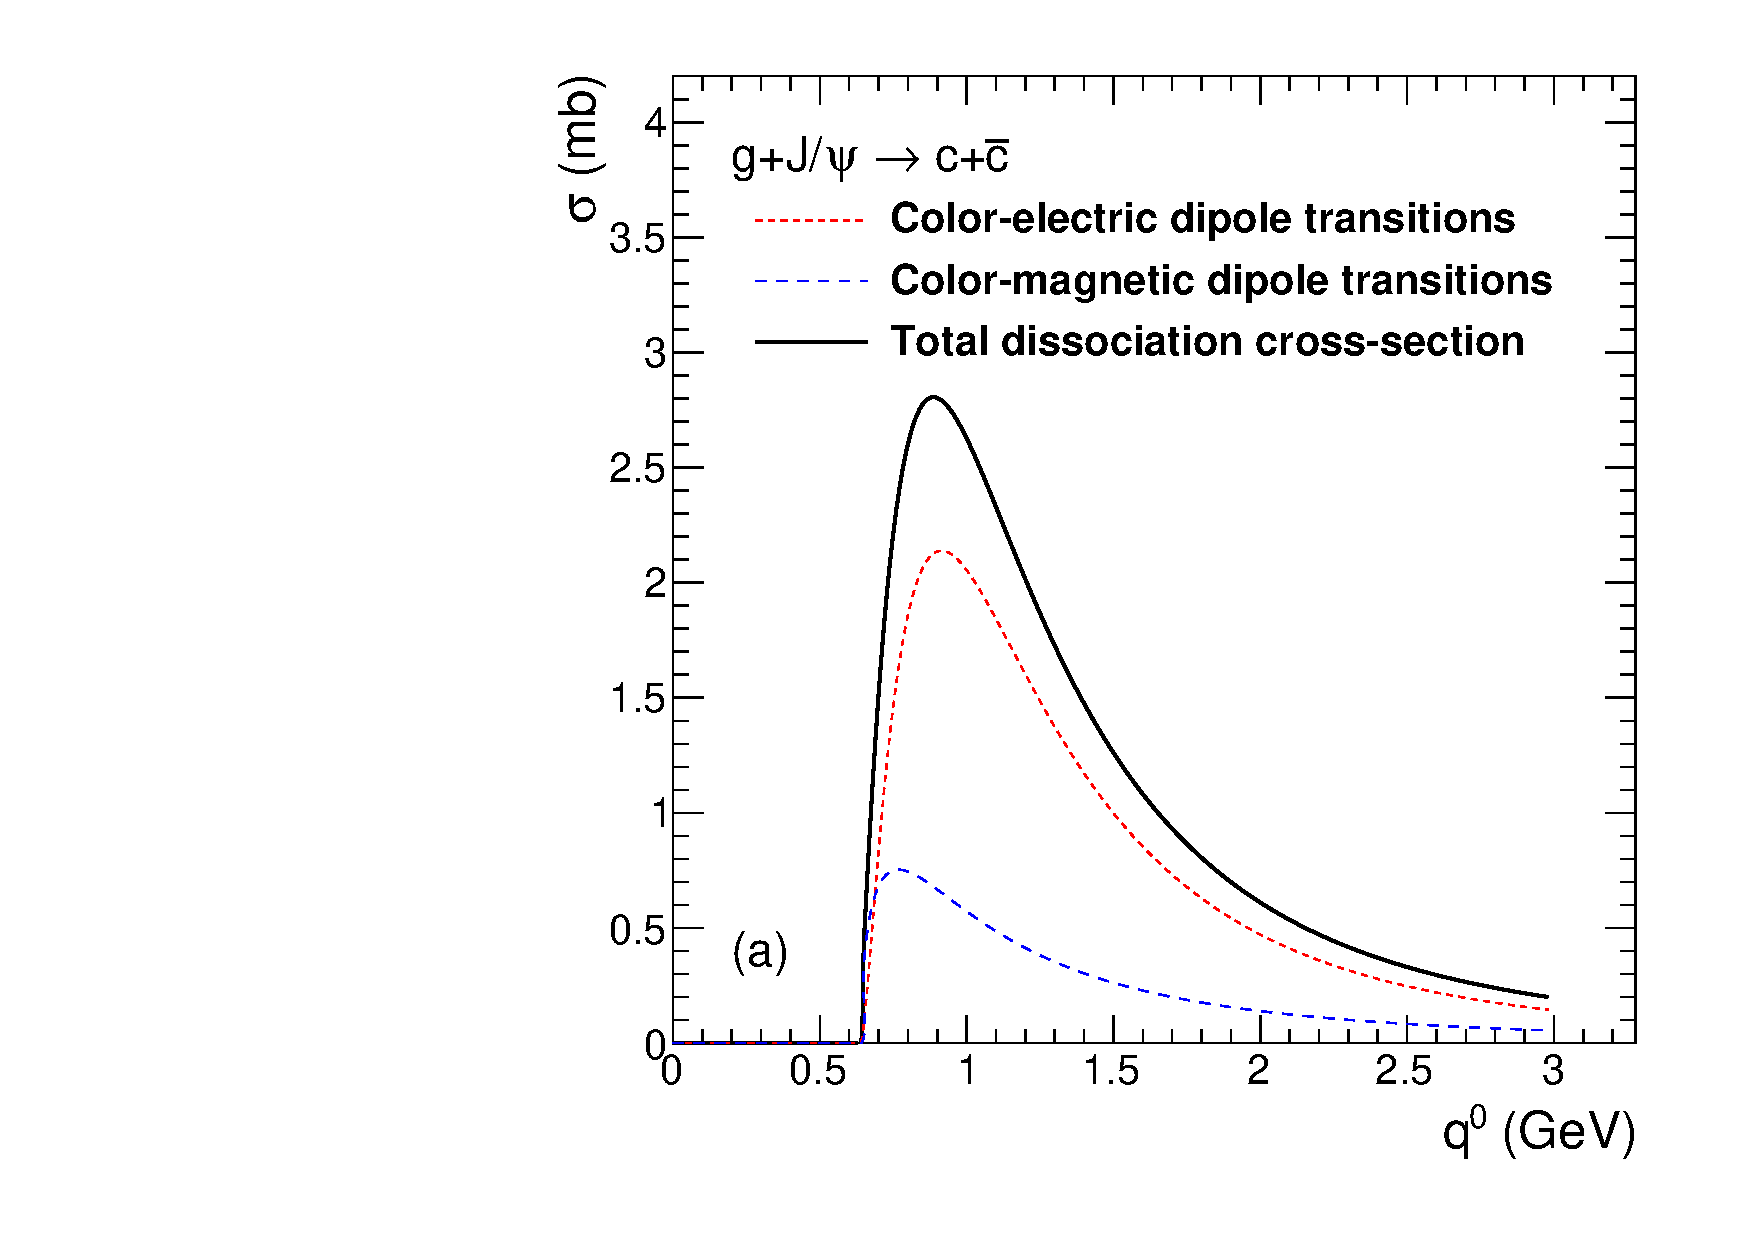
\includegraphics[width=0.49\textwidth]{Fig1a_JPsi_SigmaDq0.pdf}
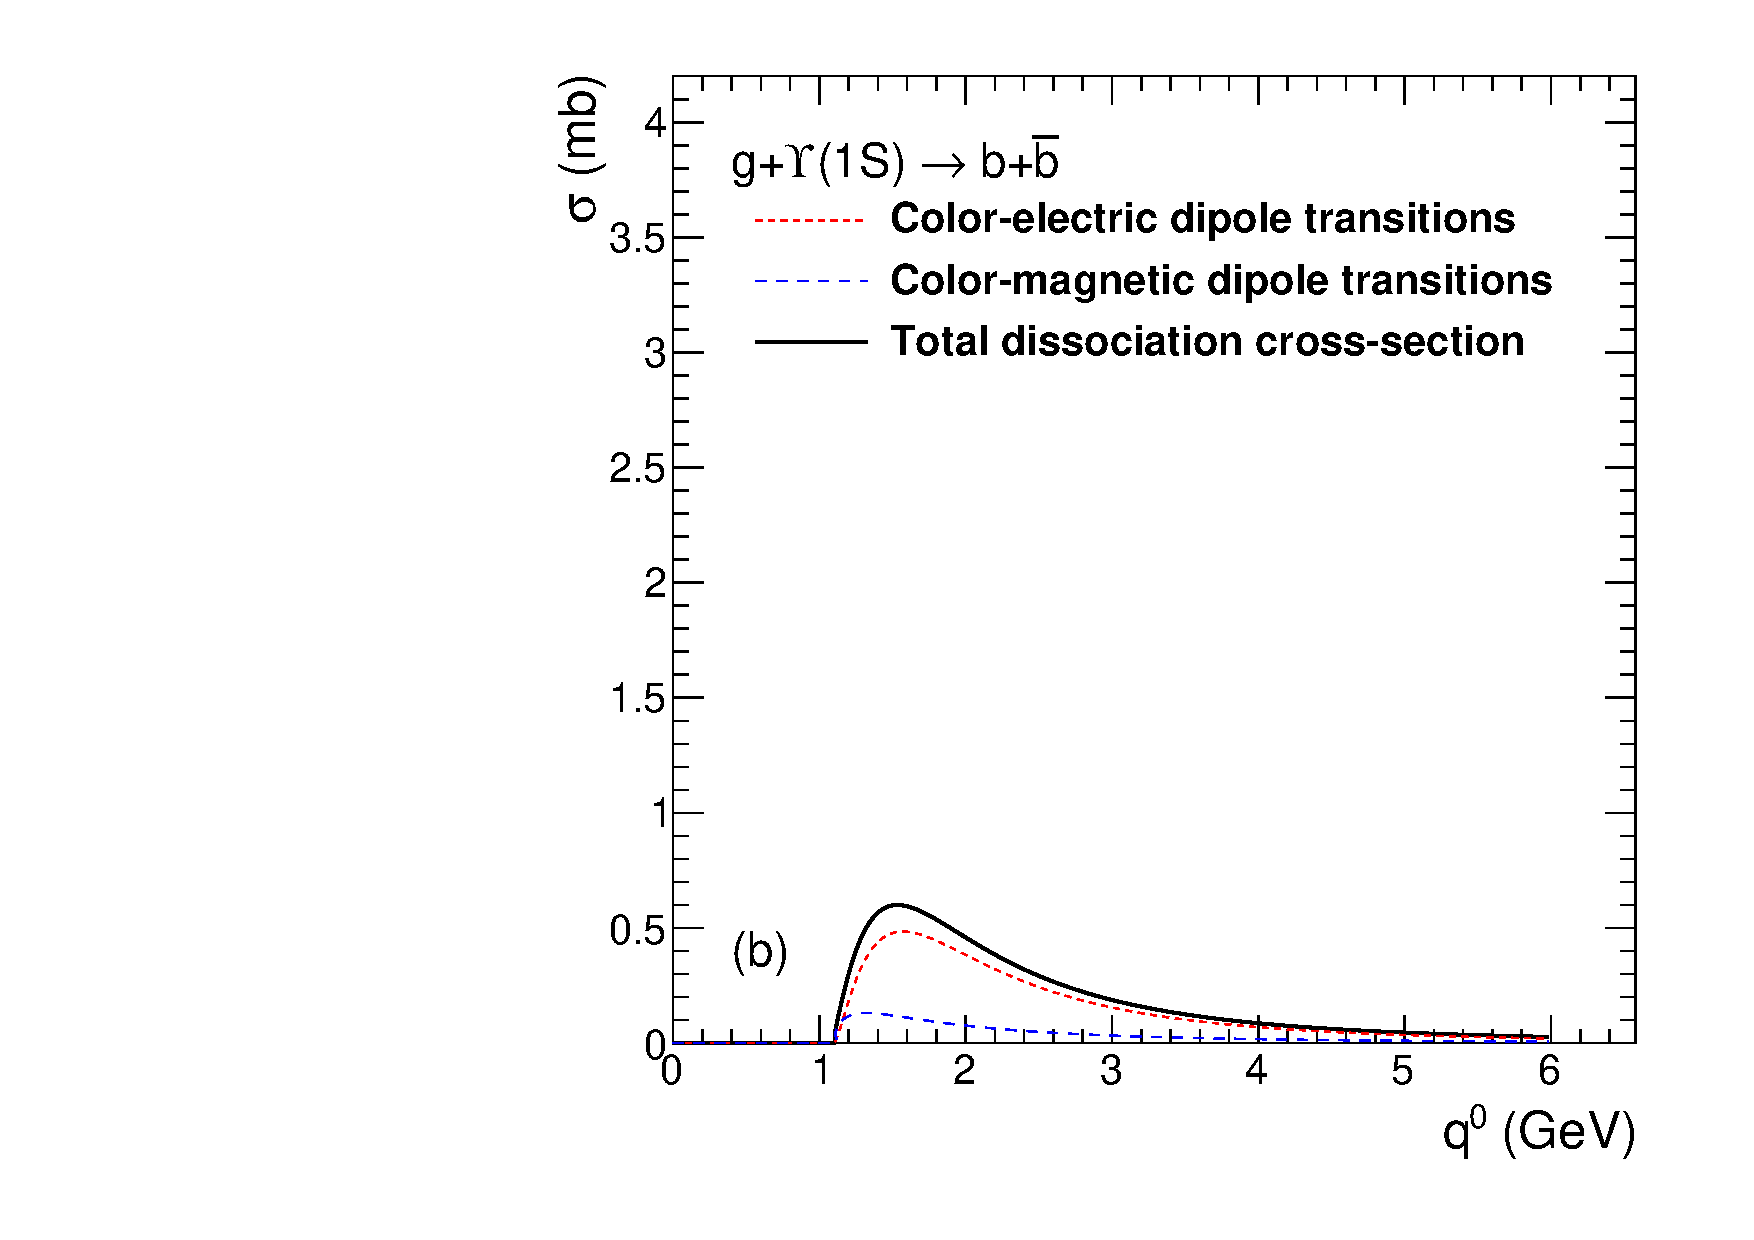
\includegraphics[width=0.49\textwidth]{Fig1b_Y1S_SigmaDq0.pdf}
\caption{(Color online) Gluon dissociation cross section of J/$\psi$ (a) and $\Upsilon$(1S) (b) as a function of gluon energy
    ($q^{0}$) in quarkonia rest frame. The total dissociation cross-section is sum of both color-electric and chromo-magnetic dipole 
    transitions.}
\label{fig:SigmaDQ0}
\end{figure}

The gluon dissociation cross section of quarkonia was calculated by
Bhanot and Peskin using operator product expansion method in the color dipole
approximation~\cite{Bhanot:1979vb}. Recently, Chen and He have revisited the
gluon dissociation using QCD multipole expansion method~\cite{Chen:2017jje}.
They reproduced the result of Ref.~\cite{Bhanot:1979vb} as the color-electric dipole (E1)
transition and also calculated the color magnetic dipole (CMD-M1) transition.
The E1 transition cross-section of gluon dissociation as a function of gluon energy, $q^0$,
in the quarkonium rest frame is~\cite{Bhanot:1979vb}
\begin{equation}
\sigma^{E1}_{D}(q^{0}) = {8\pi \over 3} \, {16^2 \over 3^2} {a_0 \over m_q}  \frac{(q^0/\epsilon_0 - 1)^{3/2}} {(q^0/\epsilon_0)^5},
\end{equation}
 where $\epsilon_0$ is the quarkonia binding energy and $m_q$ is the charm/bottom quark mass 
and $a_0=1/\sqrt{m_q\epsilon_0}$. Using the same procedure, the M1 transition cross-section of gluon 
dissociation can be calculated as~\cite{Chen:2017jje}
\begin{equation}
\sigma^{M1}_{D}(q^{0}) = {8\pi \over 3} \, {16 \over 3 } {a_0 \over m_q^{2}}  \frac{\epsilon_0(q^0/\epsilon_0 - 1)^{3/2}} {(q^0/\epsilon_0)^3},
\end{equation}
The total dissociation cross section is given as 
\begin{equation}
\sigma_D(q^0) = \sigma^{E1}_D(q^0) + \sigma^{M1}_D(q^0).
\end{equation}
The values of $\epsilon_0$ are taken as 0.64 and 1.10 GeV for the ground states, $\Jpsi$ and $\Upsilon$(1S),
respectively~\cite{Karsch:1987pv}. For the excited states of bottomonia, the dissociation cross sections are
used from Ref.~\cite{Chen:2017jje,Oh:2001rm}.

Figure \ref{fig:SigmaDQ0} shows the gluon dissociation cross sections
of $\Jpsi$ and $\Upsilon$(1S) as a function of gluon energy
for both color-electric and color-magnetic dipole transitions.
The color-magnetic dipole transition cross-section has similar shape as that of
electric cross-section and gives significant contribution 
in low and intermediate gluon energies. Total dissociation cross section increases
with gluon energy and reaches a maximum around 0.9 GeV for
J/$\psi$ and around 1.5 GeV for $\Upsilon$(1S). At higher gluon energies, the
interaction probability decreases. 
%The gluon 
%energy $q^0$ is related to the square of the center of mass energy $s$, of the quarkonium-gluon system by
%\begin{eqnarray}
% q^{0} = \frac{s-M_{Q}^{2}}{2\,M_{Q}}
%\end{eqnarray}  
%where $s=M_{Q}^{2} + 2  p_g \, \sqrt{M_{Q}^2 + p^2} - 2  p_g \, p \, {\rm cos\theta}$, and $M_{Q}$ and $p$ 
%are mass and momentum of quarkonium and $\theta$ is angle between the quarkonium and the gluon.
The dissociation rate is calculated as a function of quarkonium momentum 
by integrating the dissociation cross section over thermal gluon momentum 
distribution $f_{g}(p_g)$ as 
\begin{eqnarray}
\lambda_{D} \rho_{g}  & = & \langle \sigma v_{\rm rel} \rangle \,\rho_{g}  = \frac{g_g}{(2\pi)^{3}} \int d^{3}p_g \, f_{g}(p_g)  \, \sigma_{D}(s) v_{\rm rel}(s)  \nonumber \\ 
                   & = & \frac{g_g}{(2\pi)^{3}} \int dp_g 2\pi p_g^{2} f_{g}(p_g) \int d\,{\rm cos\theta}\,\sigma_{D}(s)\,v_{\rm rel}(s),
\label{Eqn:Diss}
\end{eqnarray}
where $\sigma_{D}(s) = \sigma_{D}(q^0(s))$. The formula in Eq.~\ref{Eqn:Diss} is assumed
for the most central collisions. We multiplied by a system size dependent factor
($\sqrt{N_{\rm part}/2A}$) to get the dissociation rate for other centralities.   
$v_{\rm rel}$ is the relative velocity, between the quarkonium and the gluon~\cite{Kumar:2014kfa}.
%The relative velocity, $v_{\rm rel}$, between the quarkonium and the gluon is
%\begin{eqnarray}
% v_{\rm rel}  = {s- M_{Q}^{2} \over 2  p_g\sqrt{M_{Q}^2 + p^2}}.  
%\label{eq7}
%\end{eqnarray}
 The $\Jpsi$ gluon dissociation rates as a function of temperature $T$ are shown in 
Fig.~\ref{fig:DRateVsTempAndPt}(a) and as a function of $p_T$ in Fig.~\ref{fig:DRateVsTempAndPt}(b).
The dissociation rate increases with temperature as the gluon density increases. 
Also, it is maximum when the quarkonium is at rest and then decreases with $p_T$.


\begin{figure}
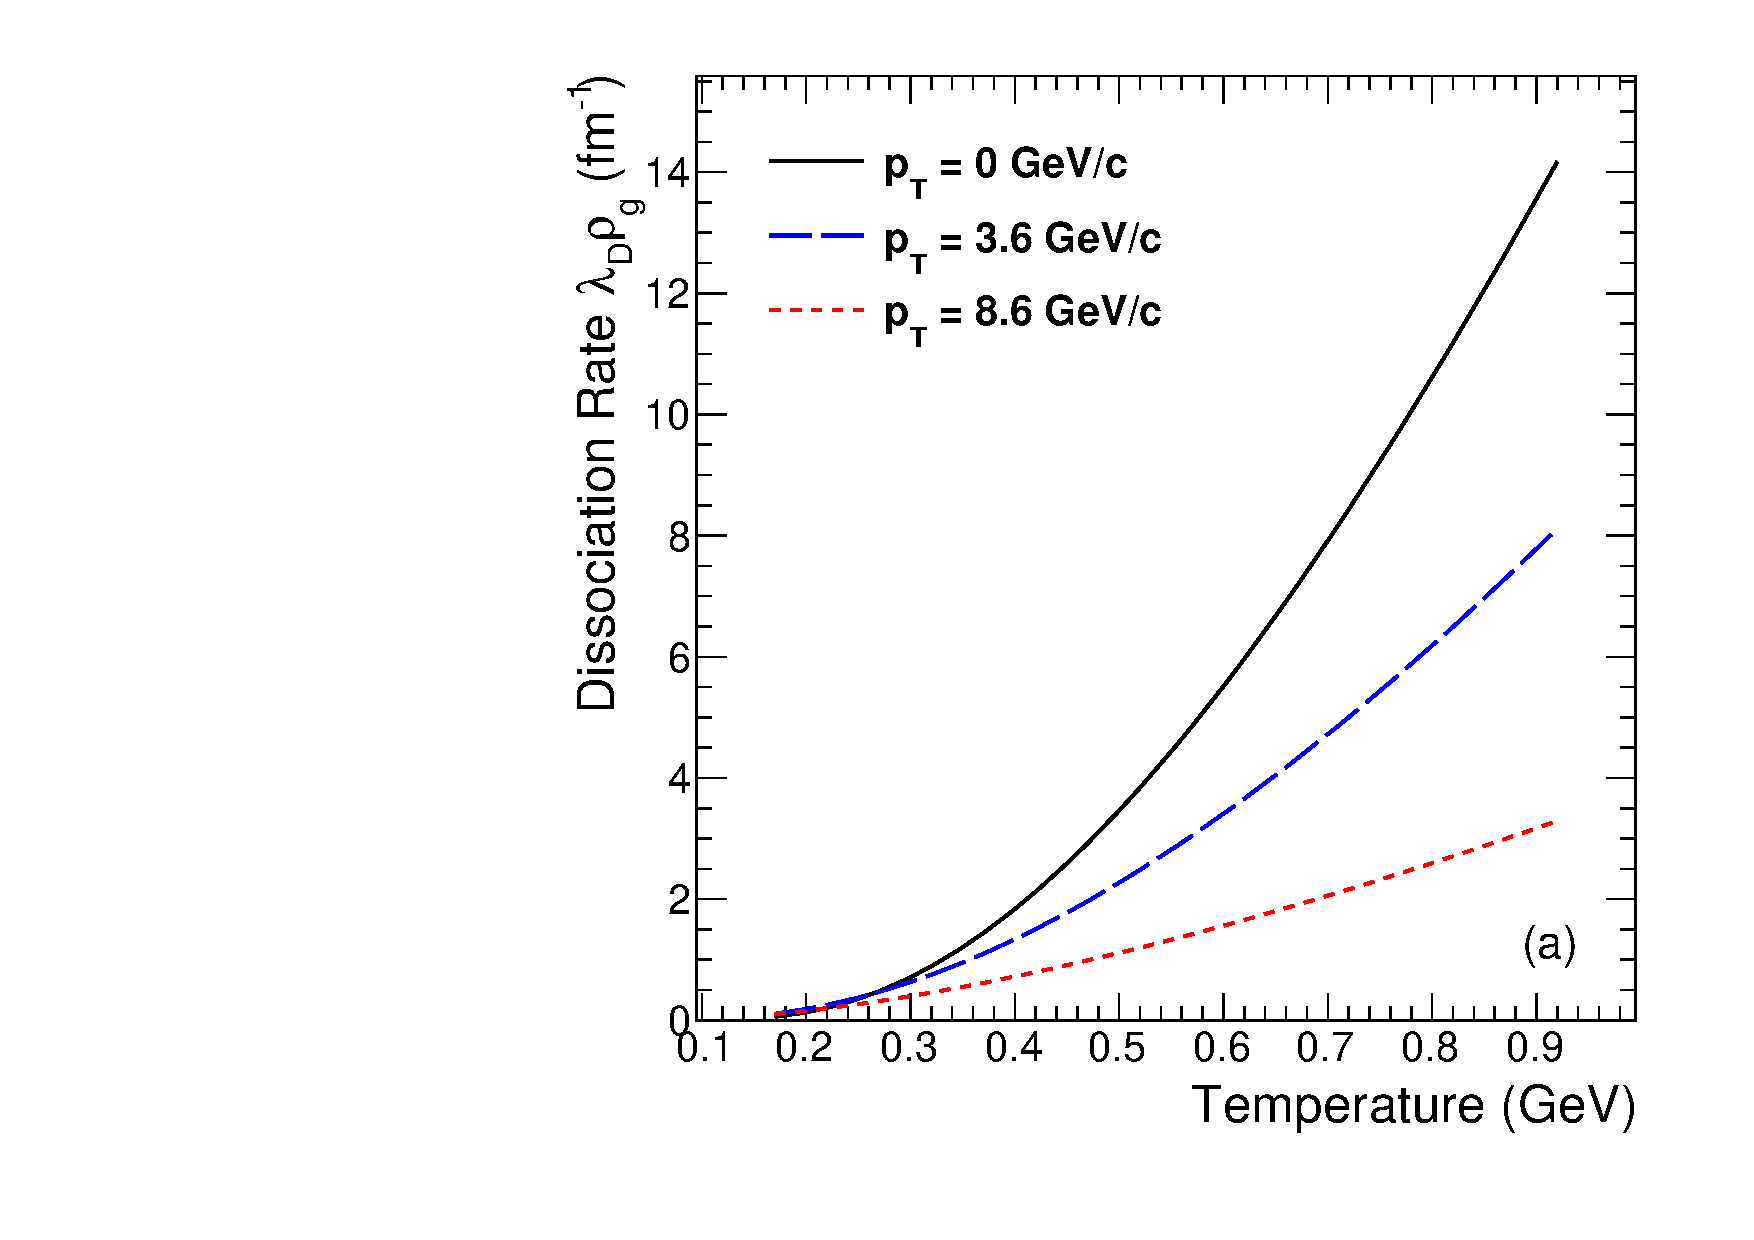
\includegraphics[width=0.49\textwidth]{Fig2a_DRateVsT.pdf}
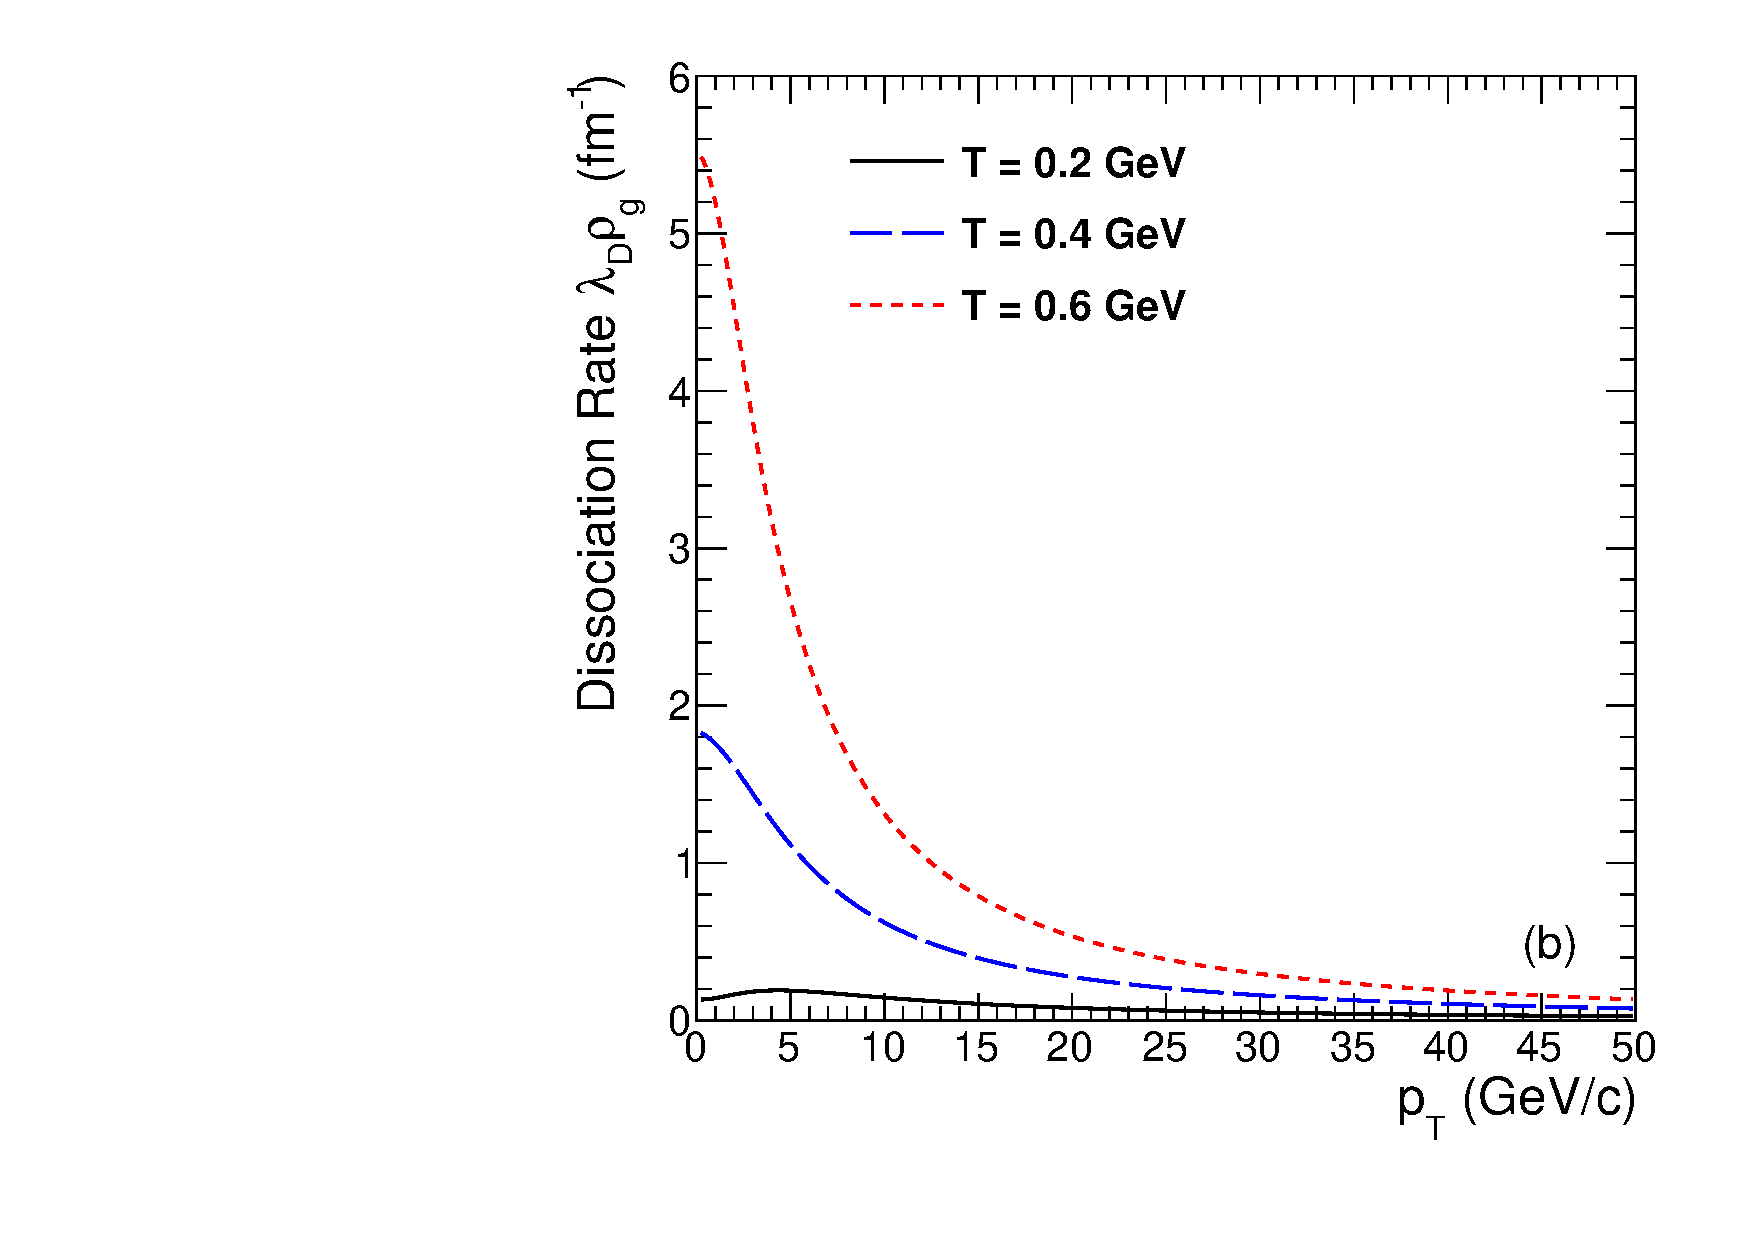
\includegraphics[width=0.49\textwidth]{Fig2b_DRateVsPt.pdf}
\caption{(Color online) Gluon dissociation rate of $\Jpsi$ as a function of (a) temperature and  
(b) $\Jpsi$ transverse momentum.}
\label{fig:DRateVsTempAndPt}
\end{figure}




We can calculate the formation cross section from the dissociation cross section
using principle of detailed balance~\cite{Thews:2000rj,Thews:2005vj} as follows
\begin{equation}
\sigma_{F} = \frac{48}{36}\,\sigma_{D}(q^0)\frac{(s-M_{Q}^2)^{2}}{s(s-4m_q^{2})}.
\end{equation}
%where $M_{Q}$ is the mass of quarkonia and $s$ is the centre of mass energy of
%of the quarkonium-gluon system.
The formation rate of quarkonium at momentum {\bf p} can be written as
\begin{equation}
\frac{d\lambda_{F}}{d{\rm\bf p}} = \int \,d^{3}p_1 \,d^{3}p_2 \,\sigma_{F}(s)\, v_{\rm rel}(s)\,f_{q}(p_1)\, f_{\bar{q}} (p_2)\,\delta({\rm\bf p}-( {\rm\bf p_1} + {\rm\bf p_2} )).
\end{equation}
Here, $f_{q/\bar{q}}(p)$ are taken as normalized near thermal distribution functions
of $q/\bar{q}$. These distributions can be described by the Tsallis
function as follows 
\begin{equation}
f_{q} (p,T) = A_{n}\,\left( 1+\frac{m_{T}}{n \,T} \right)^{-n},
\end{equation}
where $m_T\,(=\sqrt{p_{T}^{2}+m^{2}})$ is transverse mass of the heavy quark, the
power $n=14$ and $A_n$ is the normalization factor.

Figure \ref{fig:ForRateVsTempAndPt} (a) shows the behaviour of the formation rate as a function 
of temperature at different values of $\Jpsi$ meson $\pT$.
Figure~\ref{fig:ForRateVsTempAndPt} (b) shows the same as a function
of $\Jpsi$ meson $p_T$ at different temperatures.
It shows that the $\Jpsi$ generated from uncorrelated heavy quark pairs has 
softer $p_{T}$ distribution than that of $\Jpsi$'s coming from the initial hard scatterings.
Thus the effect of recombination will be important at low and intermediate $p_T$.

\begin{figure}
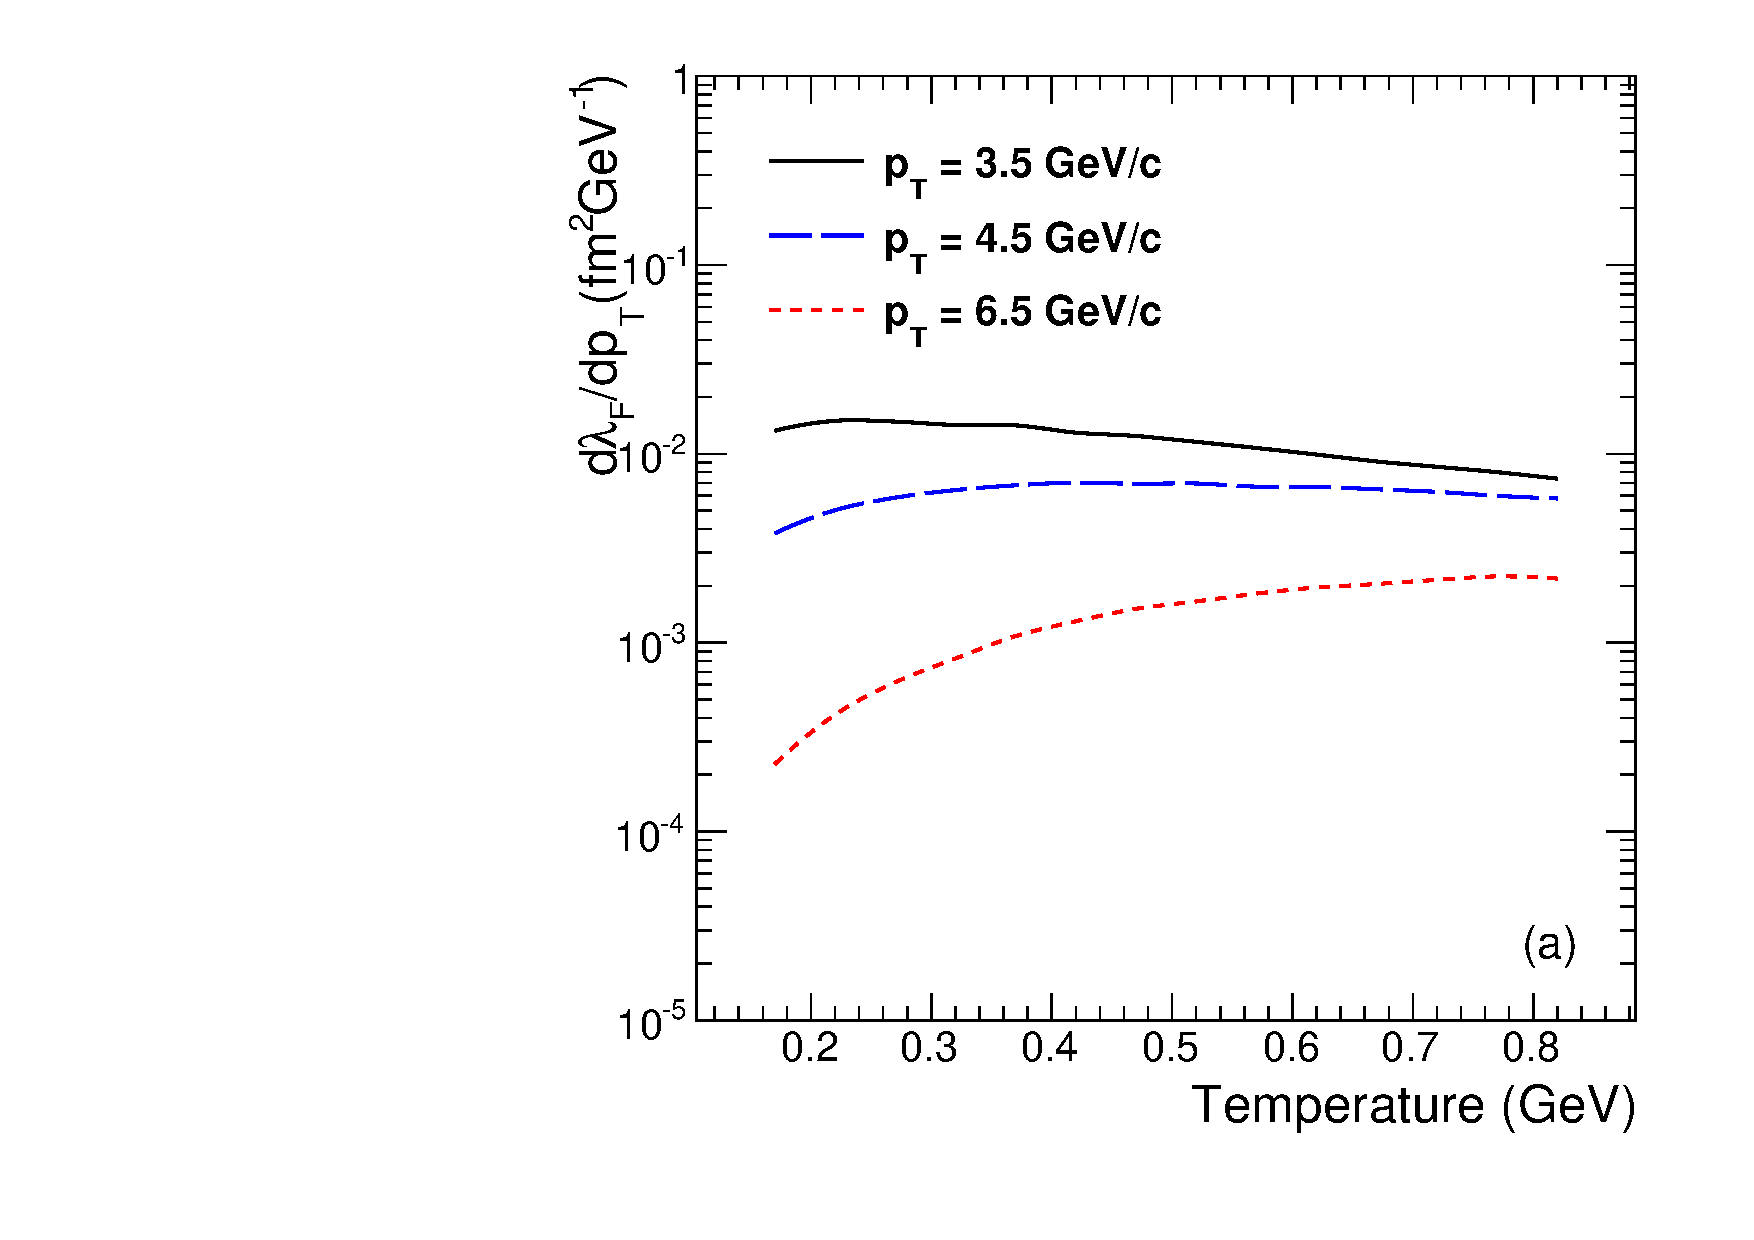
\includegraphics[width=0.49\textwidth]{Fig3a_FormRateVsT.pdf}
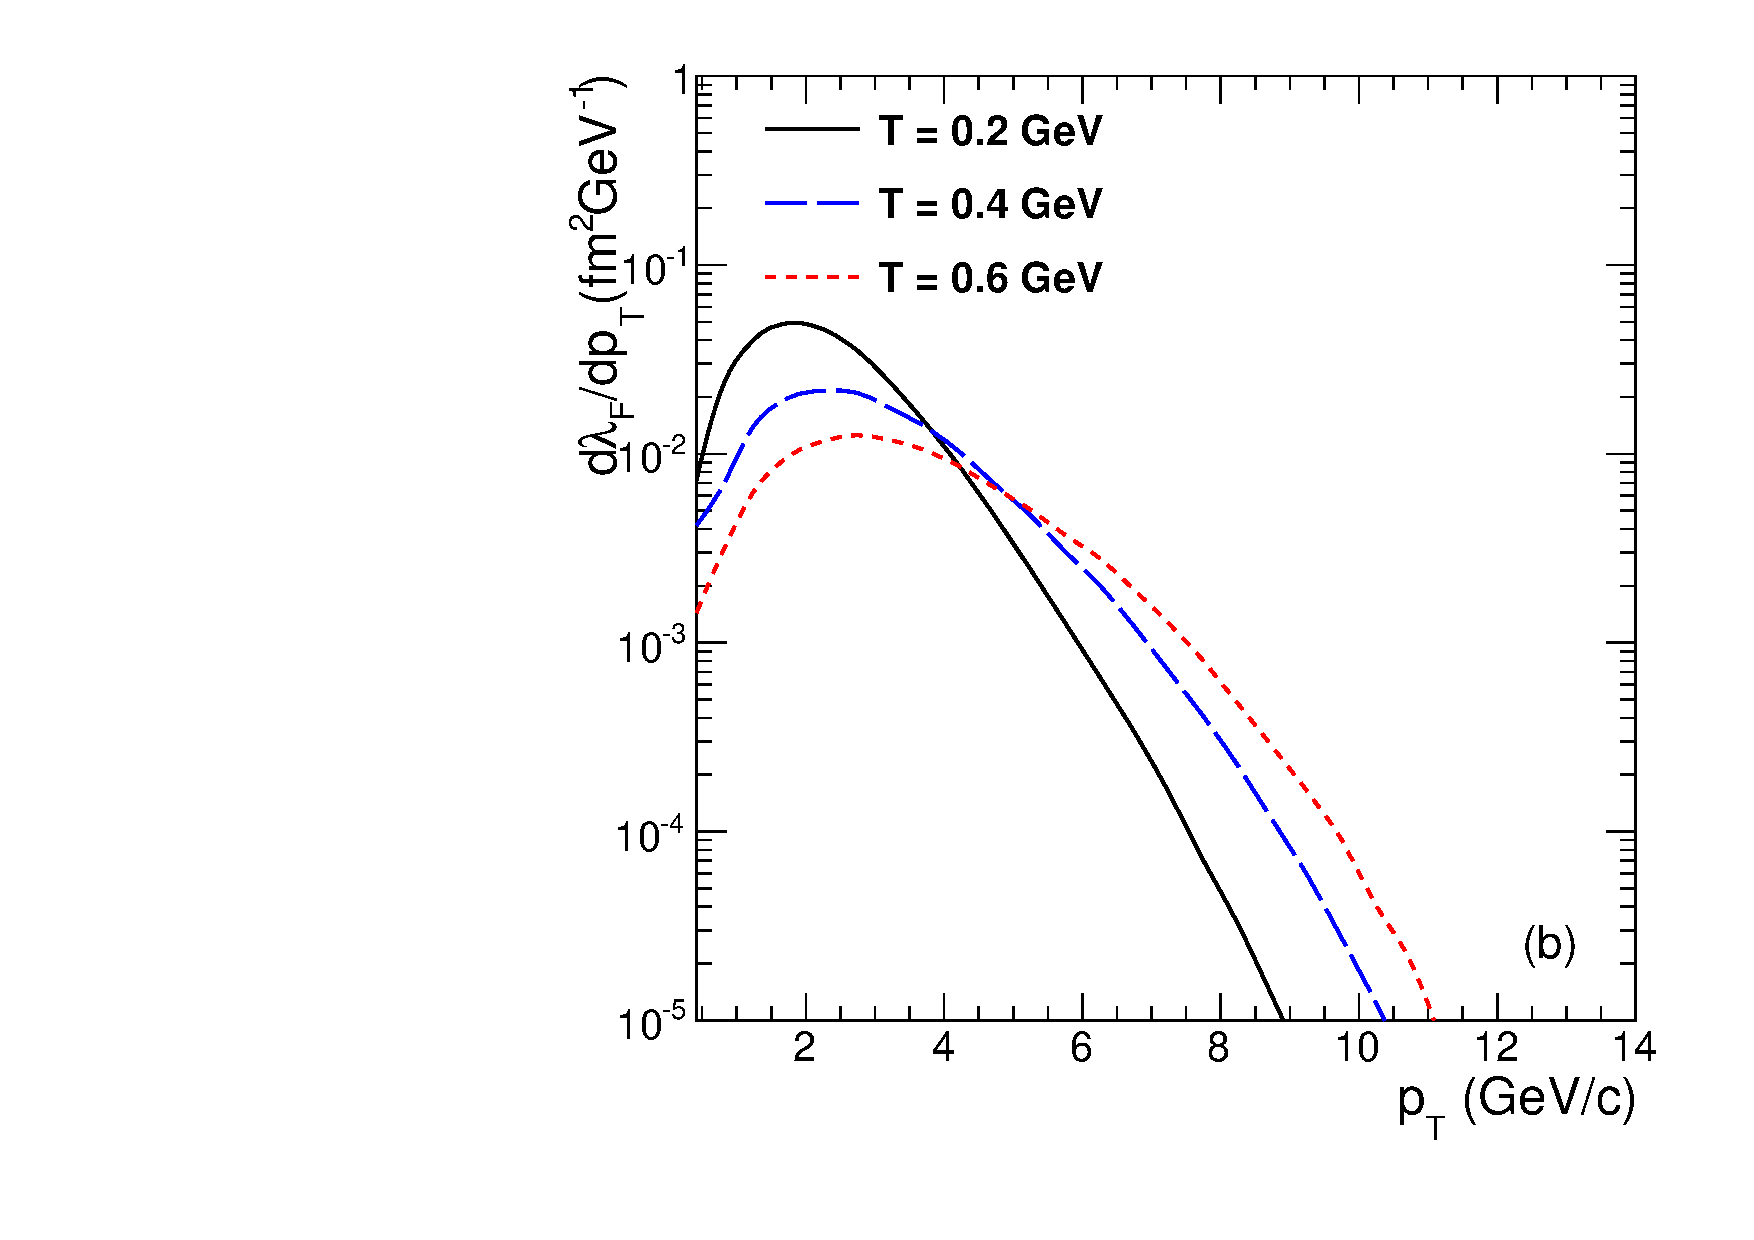
\includegraphics[width=0.49\textwidth]{Fig3b_FormRateVsPt.pdf}
\caption{(Color online) Formation rate of  $\Jpsi$ as a function of (a) temperature and 
(b) transverse momentum.}
\label{fig:ForRateVsTempAndPt}
\end{figure}


\subsection{Nuclear modification}

The nuclear modification factor ($R_{AA}$) as a function of $p_T$ can be obtained as 

\begin{equation}
  R_{AA}(p_T)= \frac{ \Sigma_{\rm Centrality} \, N_Q(p_T,N_{\rm part})}
                    { \Sigma_{\rm Centrality} \, N_{\rm coll} \, N_{Q}^{pp}(p_T)}.
\label{raa}
\end{equation}
The sum over the events is performed over the measured centrality range in the
experiment. The $\raa$ as a function of collision centrality is obtained as

\begin{equation}
  R_{AA}(N_{\rm part}) = \frac{\int_{p_{T\,\rm cut}} N_{Q}(p_T, \npart) \, p_T dp_T}
                  {\int_{p_{T\,\rm cut}} N_{\rm coll} \,\, N^{\rm pp}_{Q}(p_T) \, p_T dp_T} 
\label{raa2}
\end{equation}
Here $p_{T~{\rm cut}}$ defines the $p_T$ range for acceptance of the experiment.
and N$_{\rm coll}$ is the number of binary collisions for the centrality bins used in
experiments.
 The evolution of the system for each centrality range is governed by an isentropic
cylindrical expansion ($s(T)\,V(\tau)= s(T_0)\,V(\tau_0)$) with prescription given
in Ref.~\cite{Kumar:2014kfa}.
The equation of state (EOS) obtained by Lattice QCD and by hadronic resonances is
used~\cite{Huovinen:2009yb}. The transverse size $R$ for a given centrality
with number of participant $\npart$ is obtained as $R(\npart) = R_{A} \sqrt{\npart/2A}$,
where $R_{A}$ is radius of the nucleus.
The initial entropy density, $s(\tau_0)|_{0-5\%}$, for 0-5\% centrality is 
\begin{eqnarray}
s(\tau_0)|_{0-5\%}  = {a_{m} \over V(\tau_0)|_{0-5\%}}   \left(\frac{dN}{d\eta}\right)_{0-5\%} . 
\label{TempVsMult}
\end{eqnarray}  
Here $a_m$ (= 5) is a constant connecting the total entropy to the final hadron 
multiplicity $dN/d\eta$ obtained from hydrodynamic calculations~\cite{Shuryak:1992wc}.
%The volume element V($\tau$) is given by
%\begin{equation}
%V(\tau) = \tau\,\pi\,(R + {1\over 2} a_{T} \, \tau^2 )^{2},
%\end{equation}
%where $a_{T} = 0.1\,c^2$ fm$^{-1}$ is the transverse acceleration \cite{Kumar:2014kfa}.
The initial temperature, $T_0$, in the 0-5$\%$ most central collisions is estimated 
from the total multiplictity in the given rapidity, assuming that the initial time is
$\tau_0 = 0.3$ fm/$c$. The total multiplicity in a given rapidity window is
1.5 times the measured charged particle multiplicity in PbPb collisions at 5.02 TeV.
With the lattice EOS, at midrapidity, with $(dN_{\rm ch}/d\eta)_{0-5\%} = 1943$~\cite{Adam:2015ptt}, 
we find $T_0 = 0.516$ GeV. The freeze out temperature is taken to be $T_f=0.140$ GeV.

%%%%%%%%%%%%%%%%%%%%%%%%%%%%%%%%%%%%%%%%%%%%%%%%%%%%%%%%%%%%%%%%%%%%%%%%%%%%%%%%%%%%%%%%
\subsection{Hadronic comovers}

The suppression of quarkonia caused due to comoving pions is obtained by folding the quarkonium-pion
dissociation cross section $\sigma_{\pi Q}$ over thermal pion distributions \cite{Vogt:1988fj}. 
The  cross section of pion-quarkonia is calculated by convoluting the gluon-quarkonia cross section $\sigma_D$
over the gluon distribution obtained inside the pion~\cite{Arleo:2001mp},
\begin{equation}
\sigma_{\pi Q} (p_{\pi}) = {p_+^2 \over 2(p_\pi^2 - m_\pi^2)} \int_0^1 \, dx \, G(x) \, \sigma_D(xp_+/\sqrt {2}),
\end{equation}
where $p_+ = (p_\pi + \sqrt{p_\pi^2-m_\pi^2})/\sqrt{2}$. The term  $G(x)$ is the gluon distribution inside a pion which 
can be given by the GRV parameterization~\cite{Gluck:1991ey}. 
The comover cross section  is expected  to be small  at LHC energies~\cite{Lourenco:2008sk}.

\subsection{Experimental data to fit}

\begin{table*}[b]
\caption{Total $\ccbar$ production cross-section measured by different experiments in pp collisions at LHC.}
\begin{tabular}{l|l|l|l}
\hline 
\hline
  $\sqrt{s}$(TeV)           &$\sigma^{c\bar{c}}\pm {\rm stat.}\pm {\rm syst.}$(mb)            &Experiment      &Ref.  \\              
\hline
 2.76 TeV                   &$4.8\pm0.8^{+1.0}_{-1.3}$           & ALICE     &\cite{Abelev:2012vra}               \\
 7 TeV                      &$8.5\pm0.5^{+1.0}_{-2.4}$           & ALICE     &\cite{Abelev:2012vra}               \\
 7 TeV                      &$8.18\pm0.67^{+0.90}_{-1.62}$        & ALICE     &\cite{Adam:2016ich}               \\
 7 TeV                      &$7.13\pm0.28^{+0.90}_{-0.66}$        & ATLAS     &\cite{ATLAS:2011fea}               \\
 7 TeV                      &$8.6\pm0.3\pm0.7$                 & ATLAS     &\cite{Aad:2015zix}               \\
 7 TeV                      &$6.10\pm0.93$                    & LHCb     &\cite{LHCb:2010lga}               \\
 \hline
\hline
\end{tabular}
\label{CCBarCrossExp}
\end{table*}


















\begin{table}[t]
\caption[]{Total $\bbbar$ production cross-section measured by different experiments in pp collisions at LHC.}
\label{BBBarCrossExp}
\begin{tabular}{l|l|l|l} 
\hline 
\hline
  $\sqrt{s}$(TeV)           &$\sigma^{\bbbar}\pm {\rm stat.}\pm {\rm syst.}$($\mu$b)            &Experiment      &Ref.  \\              
\hline
 2.76 TeV                   &$130\pm15.1^{+42.1}_{-49.8}$           & ALICE     &\cite{Abelev:2014hla}               \\
 2.76 TeV                   &$162\pm14^{+55}_{-65}$                & ALICE     &\cite{Abelev:2012sca}               \\
 7 TeV                      &$383\pm21\pm116$                   & ALICE     &\cite{Abelev:2012sca}               \\
 7 TeV                      &$282\pm74^{+58}_{-68}$               & ALICE     &\cite{Abelev:2012gx}               \\
 7 TeV                      &$284\pm20^{+49}_{-49}$              & LHCb     &\cite{Aaij:2010gn}               \\
 7 TeV                      &$288\pm4^{+48}_{-48}$              & LHCb     &\cite{Aaij:2011jh}               \\
\hline
\hline
\end{tabular}
\end{table}




The total charm and total bottom production cross-sections are measured by different experiments at 
LHC~\cite{Abelev:2012vra,Adam:2016ich,ATLAS:2011fea,Aad:2015zix,LHCb:2010lga,Abelev:2014hla,Abelev:2012sca,Abelev:2012gx,Aaij:2010gn,Aaij:2011jh}. 
Table~\ref{CCBarCrossExp} and Table~\ref{BBBarCrossExp} show the values of total $\ccbar$ 
and $\bbbar$ production cross-section measured in pp collisions at LHC.
We use these values to estimate the 
total heavy quark production cross section at $\sNN =$ 5.02 TeV.
The quarkonium production cross sections are calculated from the measured heavy 
quark production cross-section using the energy independent factors obtained
from the color evaporation model~\cite{Kumar:2014kfa,Nelson:2012bc,Vogt:2012vr}.
%The quarkonium production cross sections are then determined using the factor
%from the color evaporation model~\cite{Nelson:2012bc,Vogt:2012vr}.
The cold nuclear matter (CNM) effects i.e. the modifications of the parton distribution
functions (nPDF) in PbPb collisions is calculated using the central EPS09 NLO
parameter set~\cite{Eskola:2009uj} .
The uncertainty in cold matter effects is obtained by adding the EPS09 NLO uncertainties in quadrature.

The production cross sections for heavy flavor and quarkonia at $\sNN =$ 5.02 
TeV are given in Table~\ref{Tab:NLOcross}.  The yields in a minimum bias 
PbPb event is obtained from the per nucleon cross
section, $\sigma_{\rm PbPb}$ as 
%\begin{eqnarray}
%N = {A^2 \sigma_{\rm PbPb} \over  
%\sigma_{\rm PbPb}^{\rm tot}} \, \, .
%\end{eqnarray}
\begin{eqnarray}
  N = \frac{A^2 \sigma_{\rm PbPb}}{\sigma_{\rm PbPb}^{\rm tot}} \, \, .
\end{eqnarray}
At 5.02 TeV, the total PbPb cross section, $\sigma_{\rm PbPb}^{\rm tot}$, 
is 7.7 b \cite{Chatrchyan:2011sx}.










\begin{table}
\caption[]{ Heavy quark and quarkonia production  cross sections per nucleon pair at
  $\sqrt{s_{_{_{NN}}}}= 5.02$ TeV. The quantity $N^{\rm PbPb}$ gives the initial number of
  heavy quark pair/quarkonia in one PbPb event.}
\label{Tab:NLOcross}
\begin{tabular}{l|l|l|l|l} 
\hline 
\hline
             &$ c \overline c$            &$\Jpsi$                      & $ b \overline b$                    & $\Upsilon$   \\              
\hline
$\sigma_{pp}$  &$6.754\pm0.641$ mb     & $35.32\pm3.35~\mu$b     & $210.30\pm46.21~\mu$b            & $0.4206\pm0.0924~\mu$b  \\


$\sigma_{\rm PbPb}$ &$4.669\pm0.443$ mb    &$24.56\pm2.33~\mu$b    & $179.30\pm0.39.40~\mu$b             &$0.3586\pm0.0788~\mu$b  \\


$N^{\rm PbPb}$     &$26.23\pm3.35$       & $0.1381\pm0.0131$         & $1.007\pm0.221$                  & $0.0020\pm0.0004$       \\

\hline
\hline
\end{tabular}
\end{table}






\section{Results and discussions}


\begin{figure}
\begin{minipage}{1.0\linewidth}
\centering
{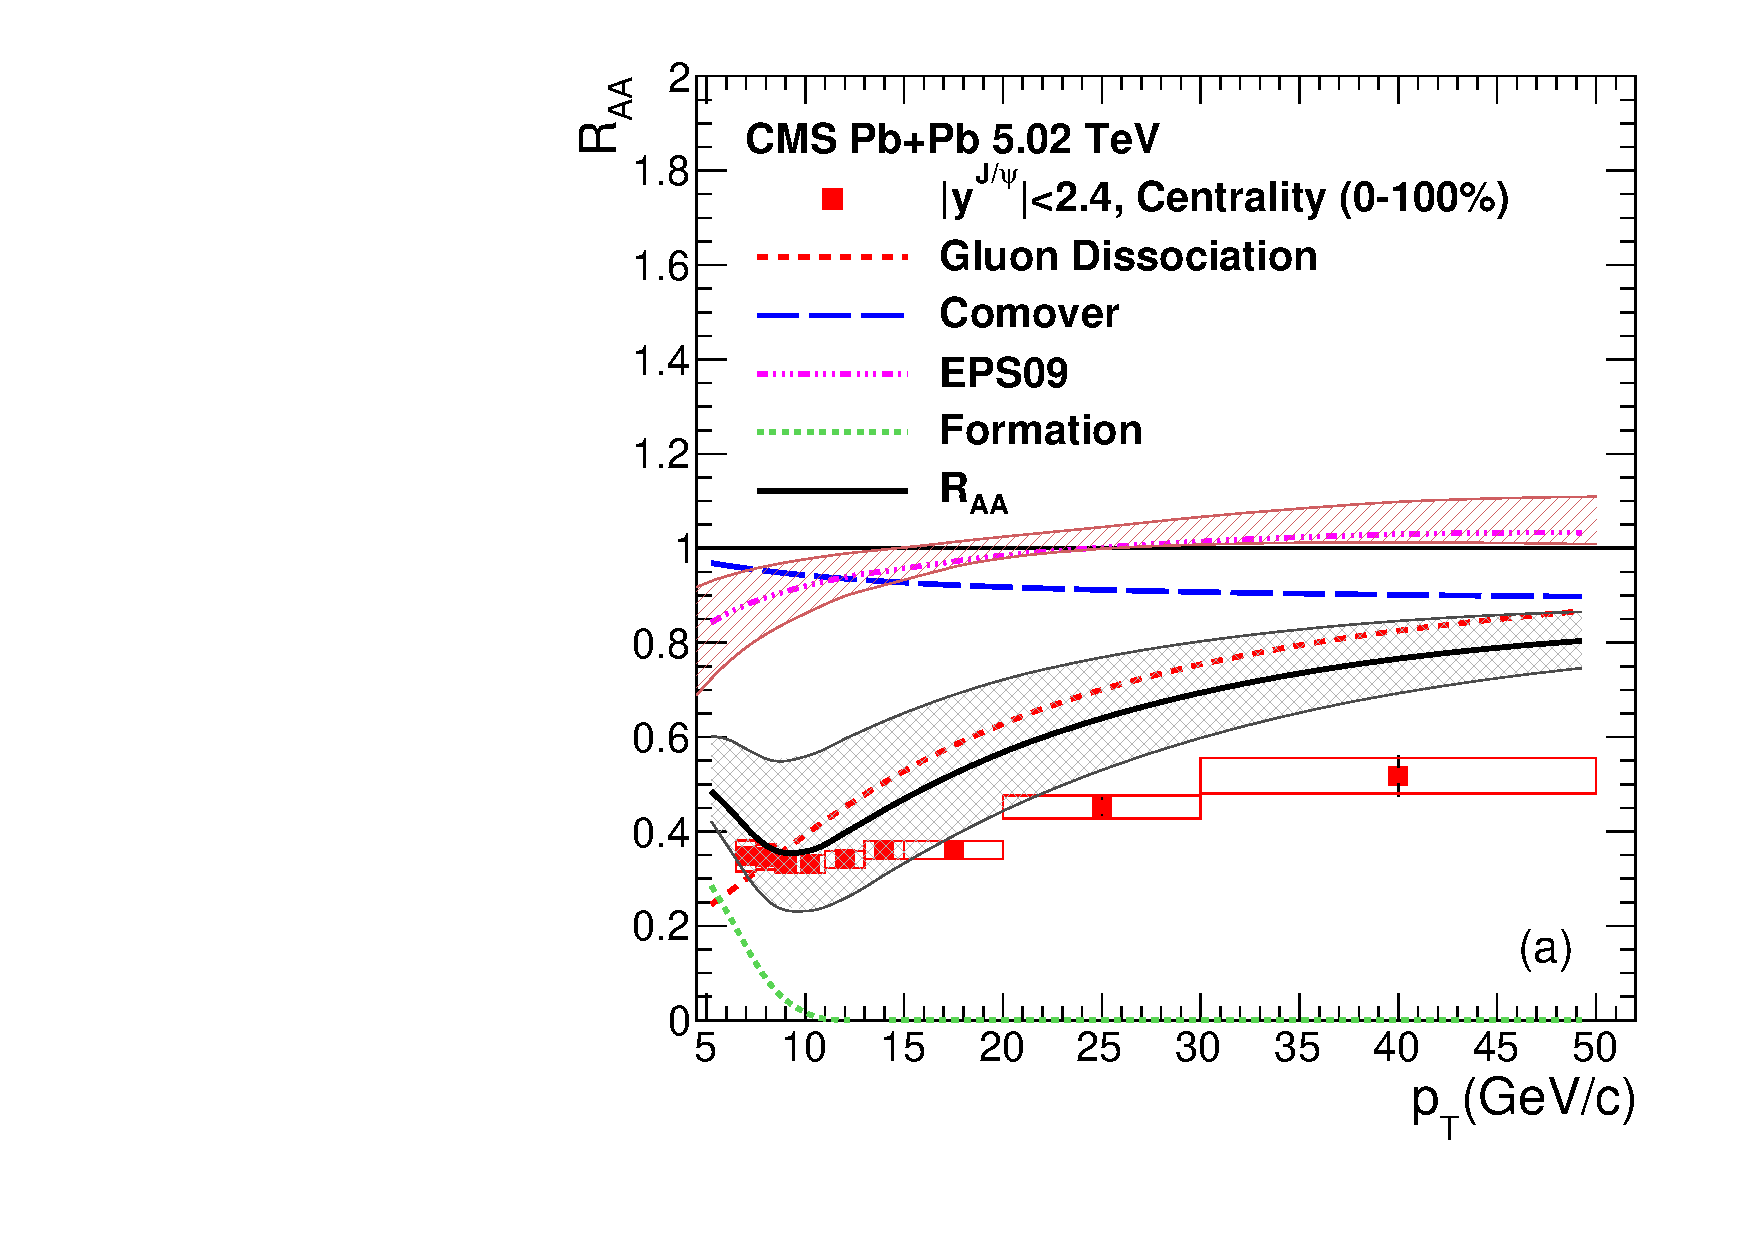
\includegraphics[width=0.49\textwidth]{Fig4a_CMS_RAAPt_Shade.pdf}}
{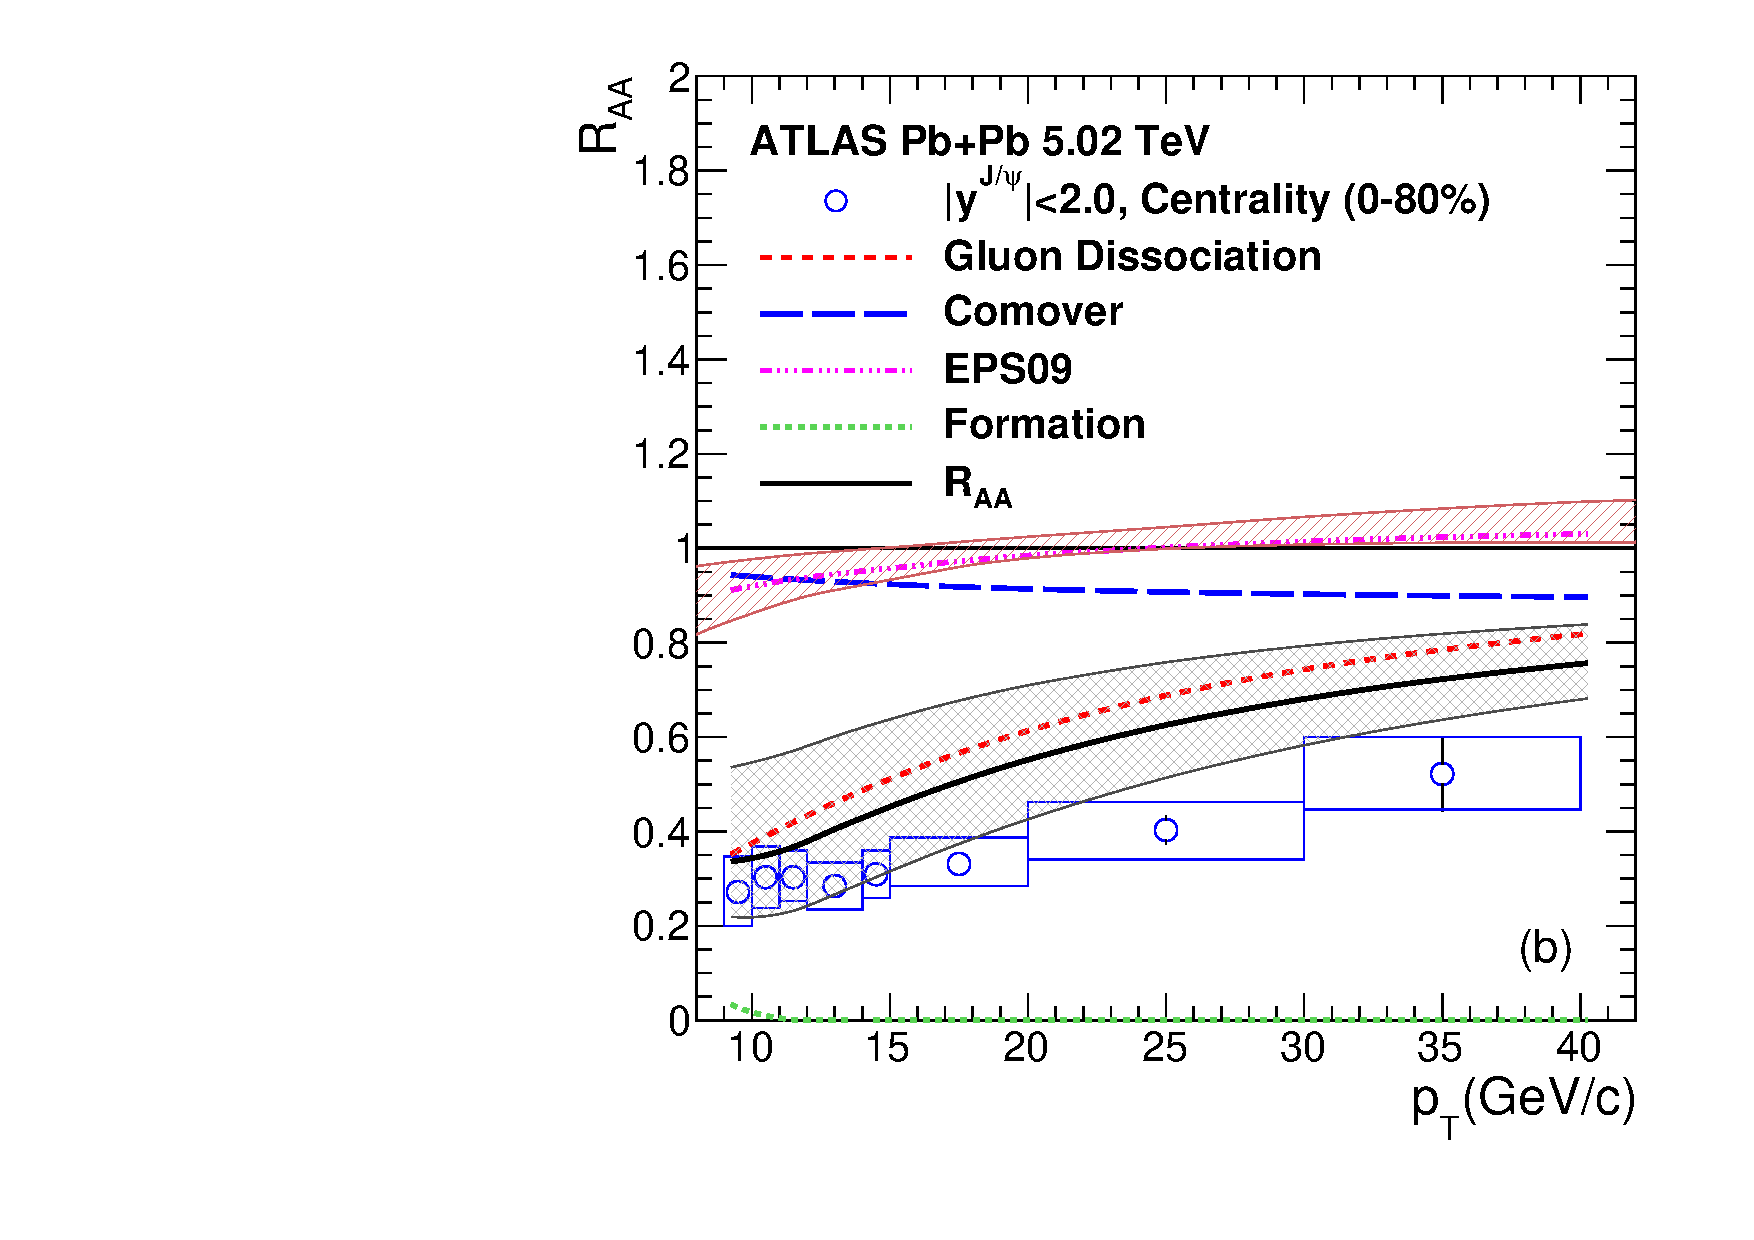
\includegraphics[width=0.49\textwidth]{Fig4b_ATLAS_RAAPt_Shade.pdf}}
\end{minipage}%
\ \\
\centering
\begin{minipage}{0.5\linewidth}
\centering
{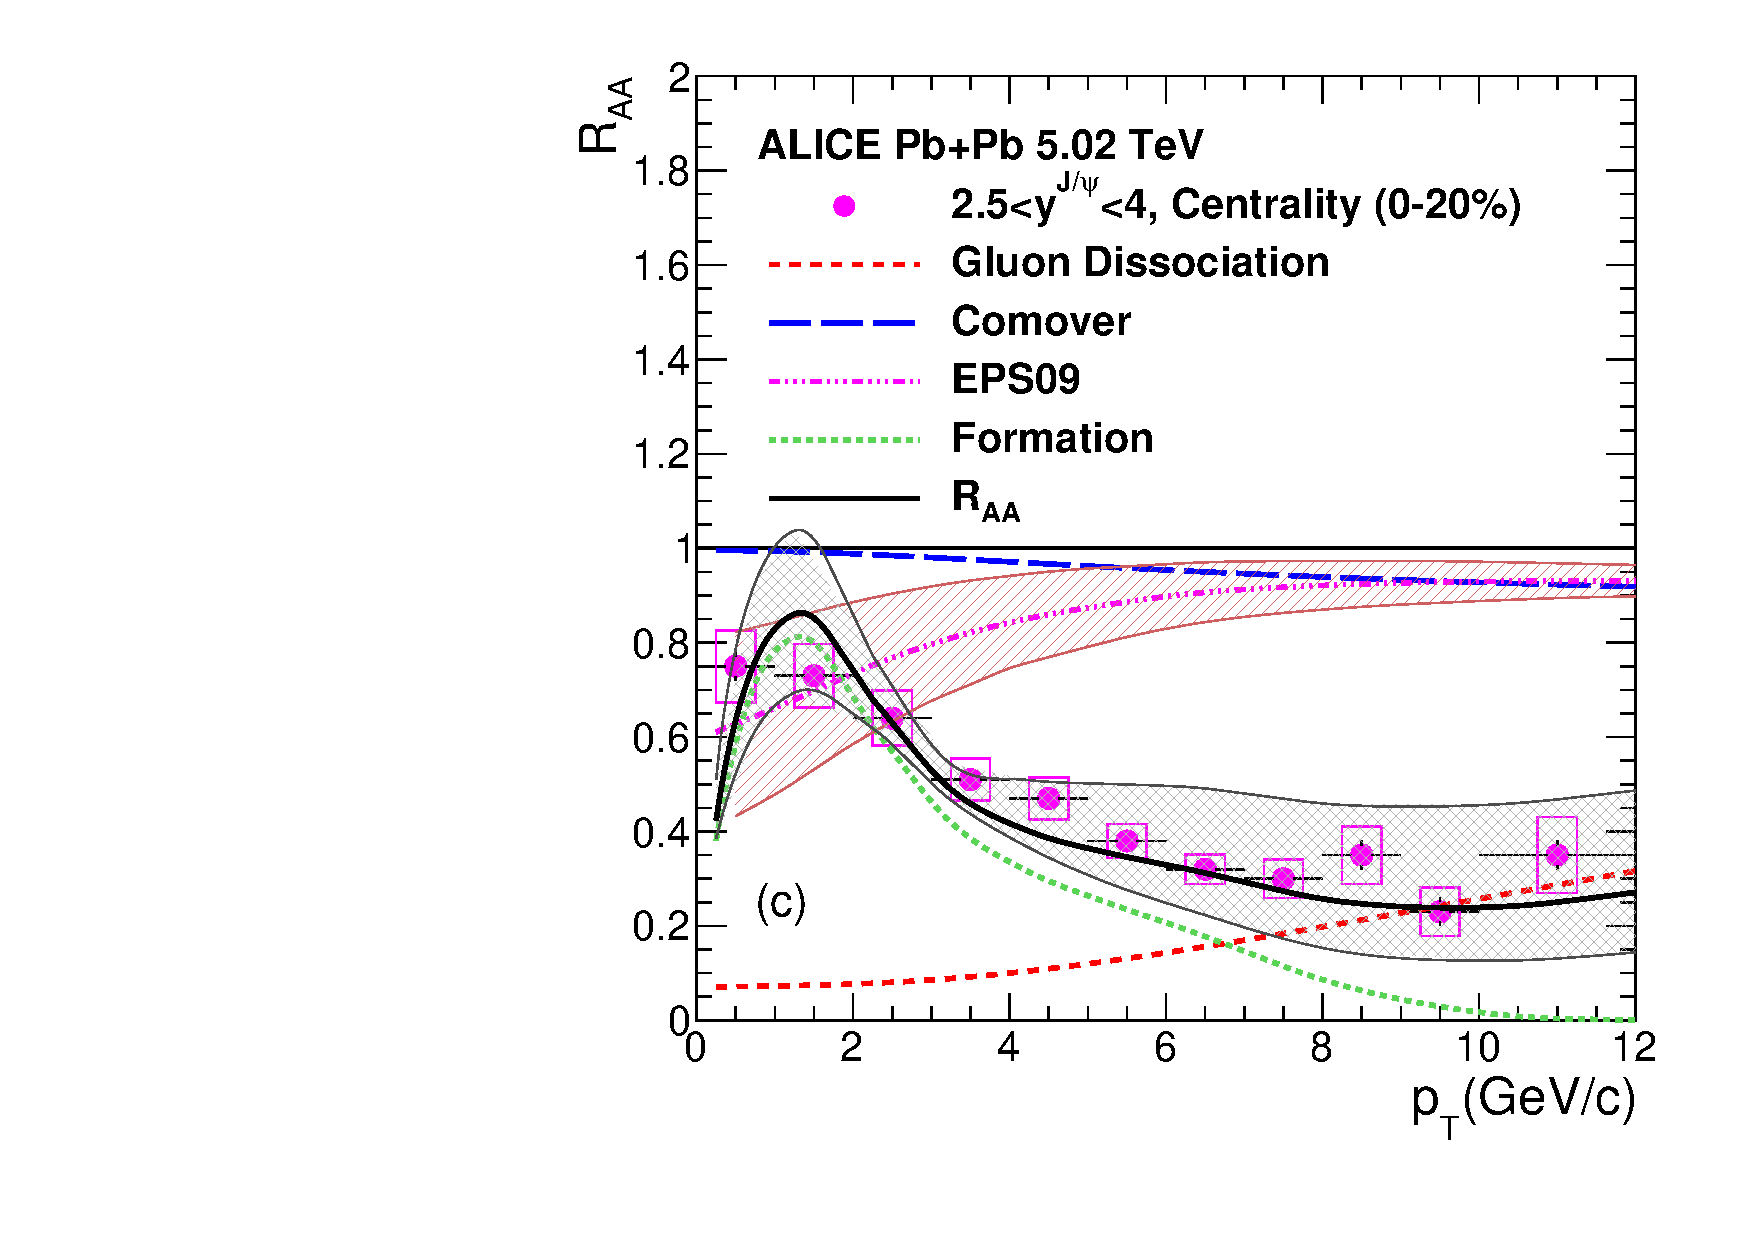
\includegraphics[width=1.0\textwidth]{Fig4c_ALICE_RAAPt_Shade.pdf}}
\end{minipage}%
\caption{(Color online)
Calculated nuclear modification factor ($R_{AA}$) as a function of $\Jpsi$ 
transverse momentum compared with (a) CMS, (b) ATLAS and (c) ALICE
measurements~\cite{Sirunyan:2017isk,ATLAS:2016qpn,Adam:2016rdg}.}
\label{fig:JPsiRaaVsPt}
\end{figure}



\begin{figure}
\begin{minipage}{1.0\linewidth}
\centering
{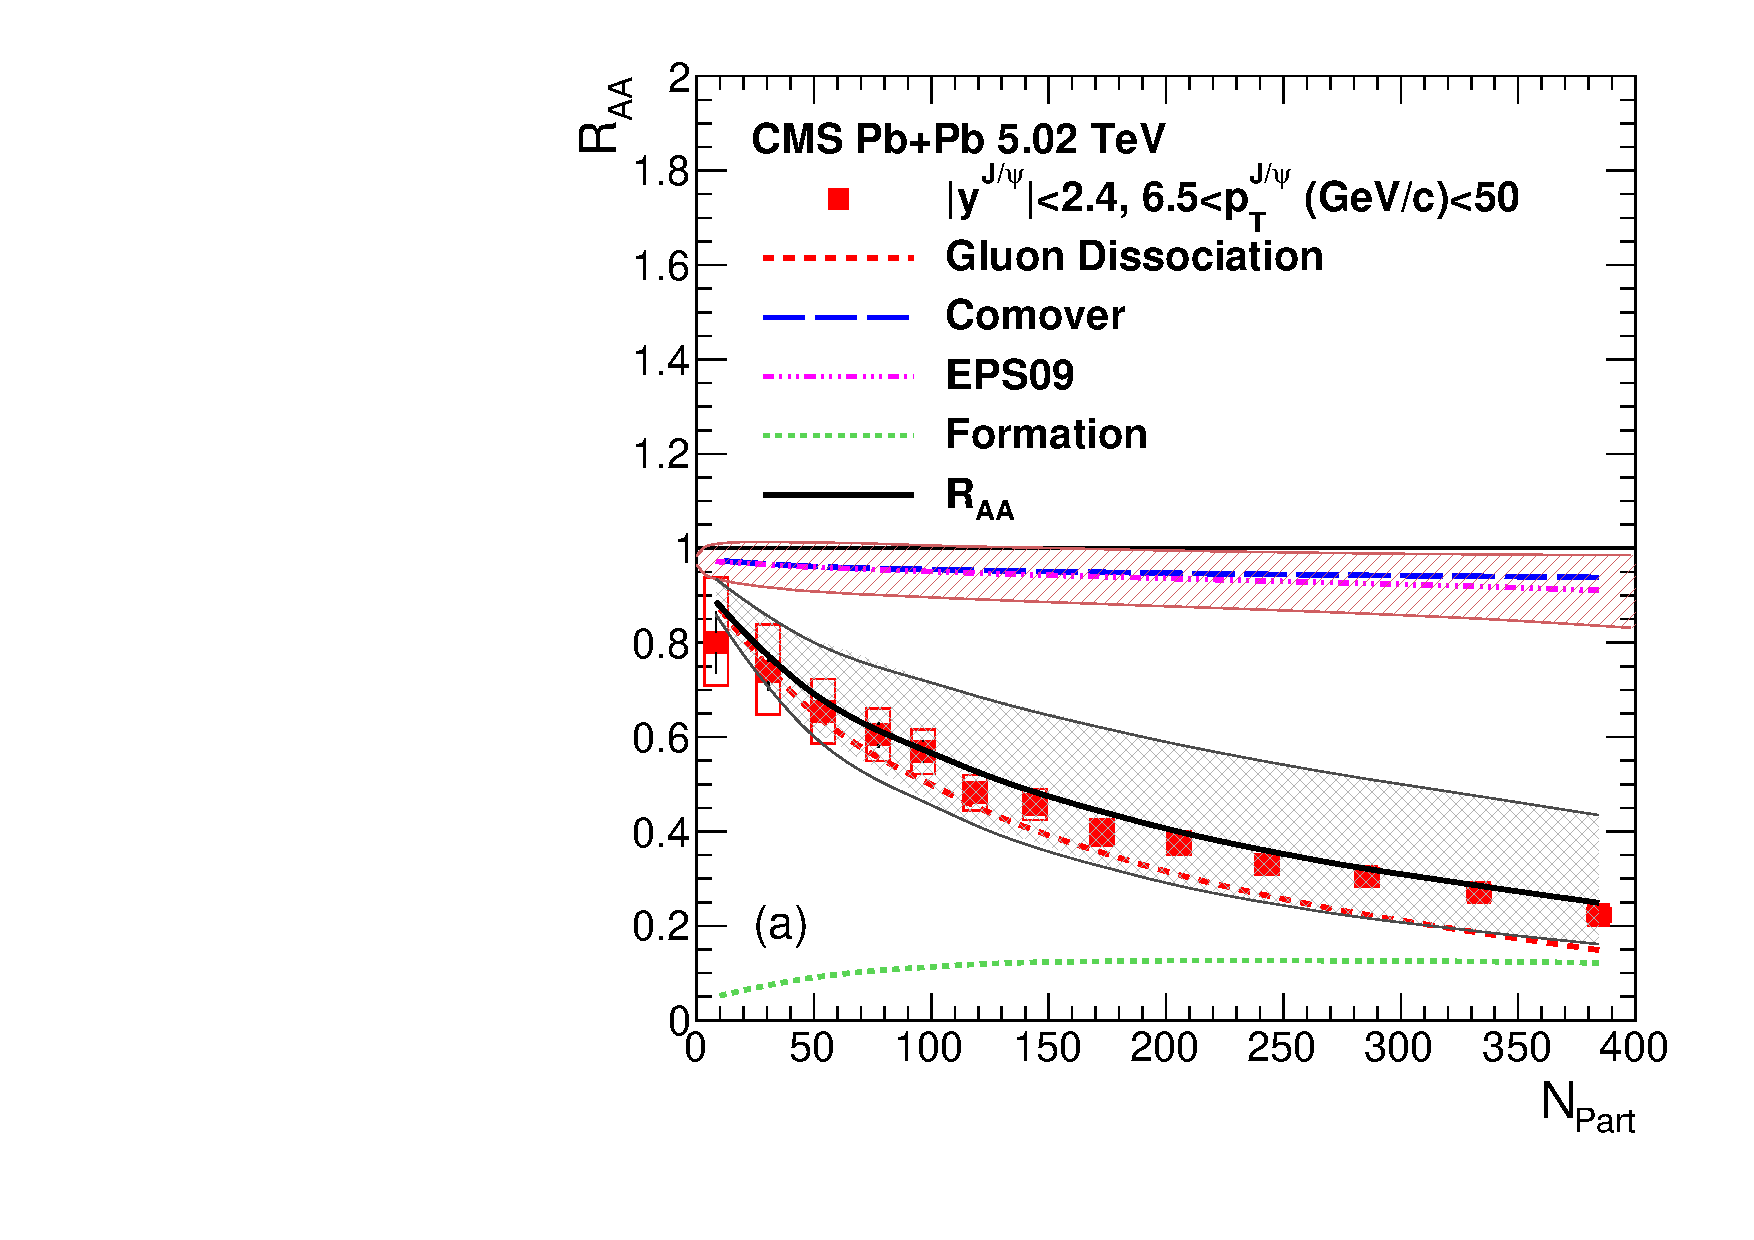
\includegraphics[width=0.49\textwidth]{Fig5a_CMS_RAANPart_Shade.pdf}}
{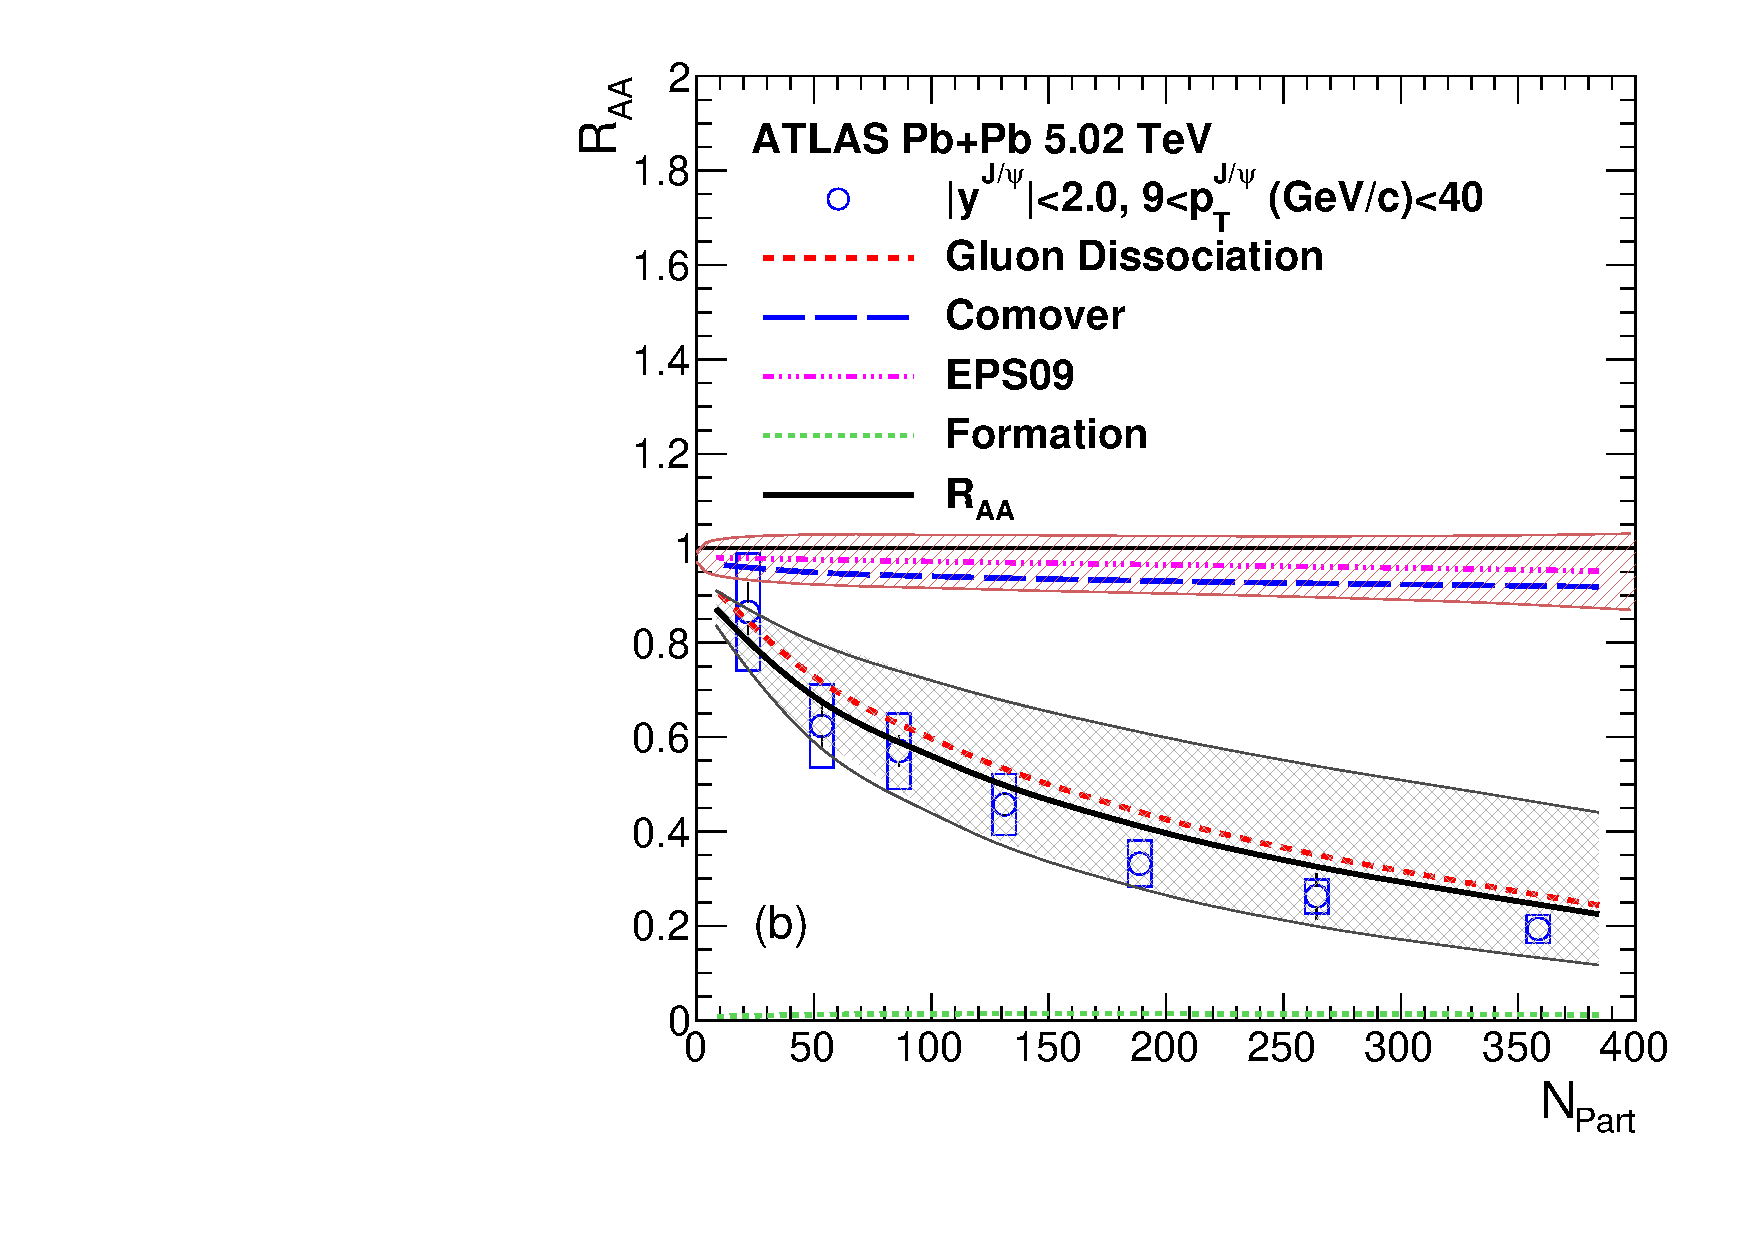
\includegraphics[width=0.49\textwidth]{Fig5b_ATLAS_RAANPart_Shade.pdf}}
\end{minipage}%
\ \\
\centering
\begin{minipage}{0.5\linewidth}
\centering
{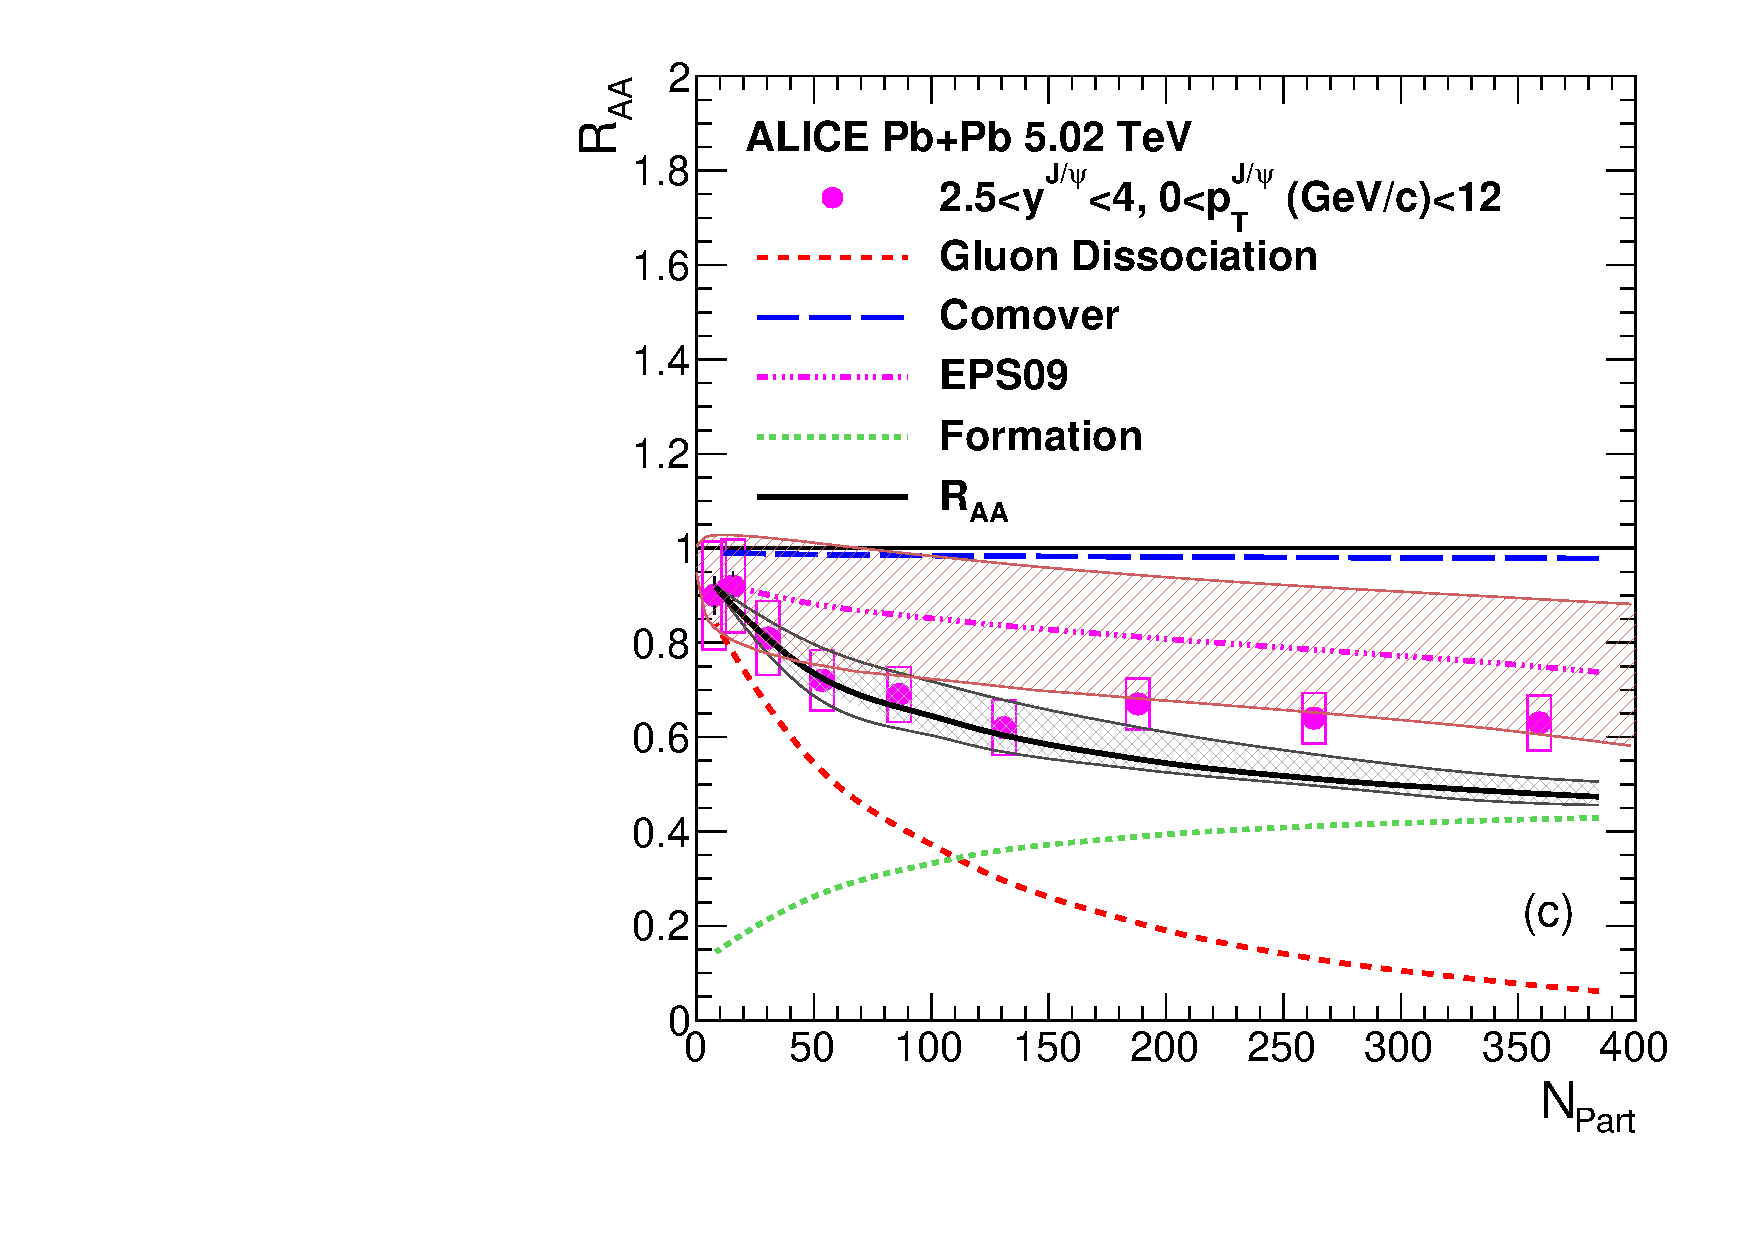
\includegraphics[width=1.0\textwidth]{Fig5c_ALICE_RAANPart_Shade.pdf}}
\end{minipage}%
\caption{(Color online) Calculated nuclear modification factor ($R_{AA}$) of $\Jpsi$ as a function
  of centrality of collisions, compared with (a) CMS, (b) ATLAS and (c) ALICE
  measurements~\cite{Sirunyan:2017isk,ATLAS:2016qpn,Adam:2016rdg}.}
\label{fig:JPsiRaaVsNPart}
\end{figure}






\begin{figure}
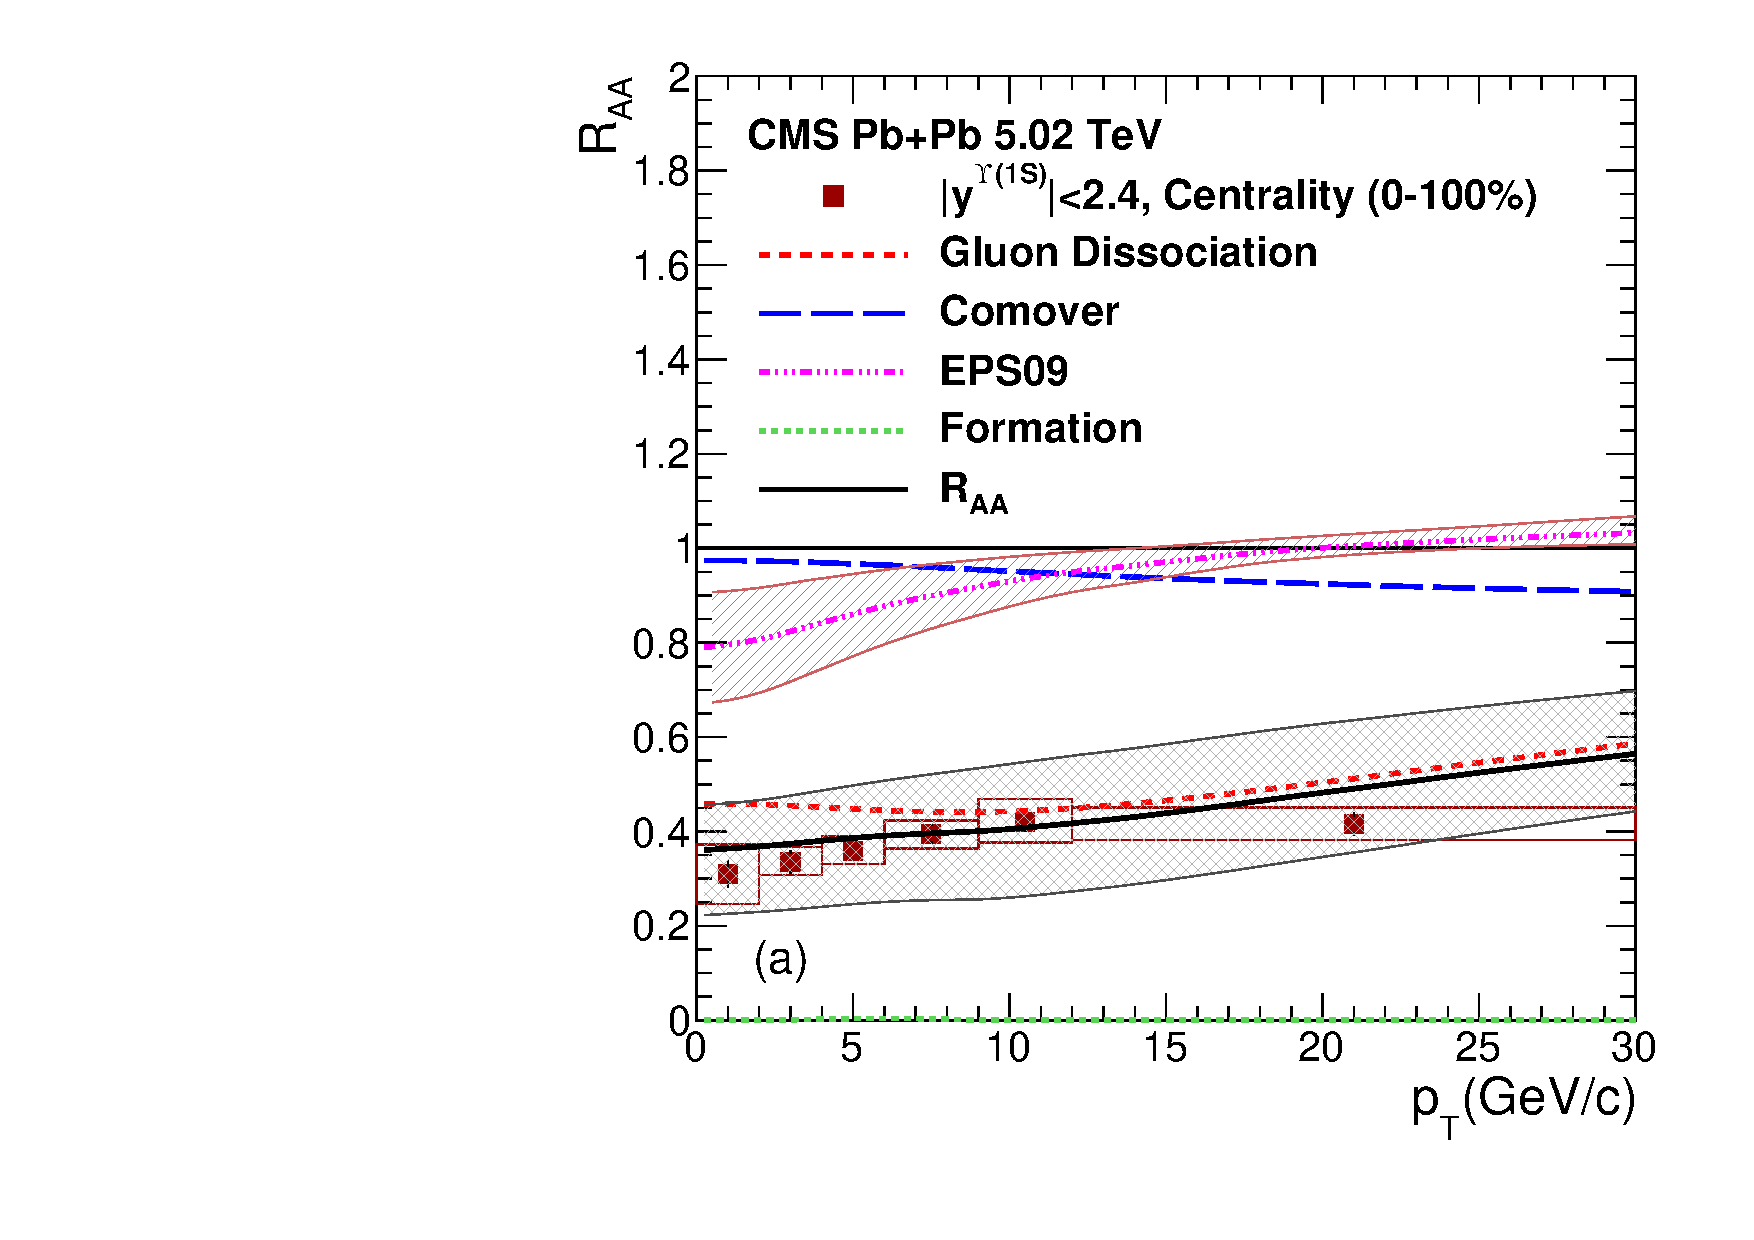
\includegraphics[width=0.49\textwidth]{Fig6a_Y1S_CMS_RAAPt_Shade.pdf}
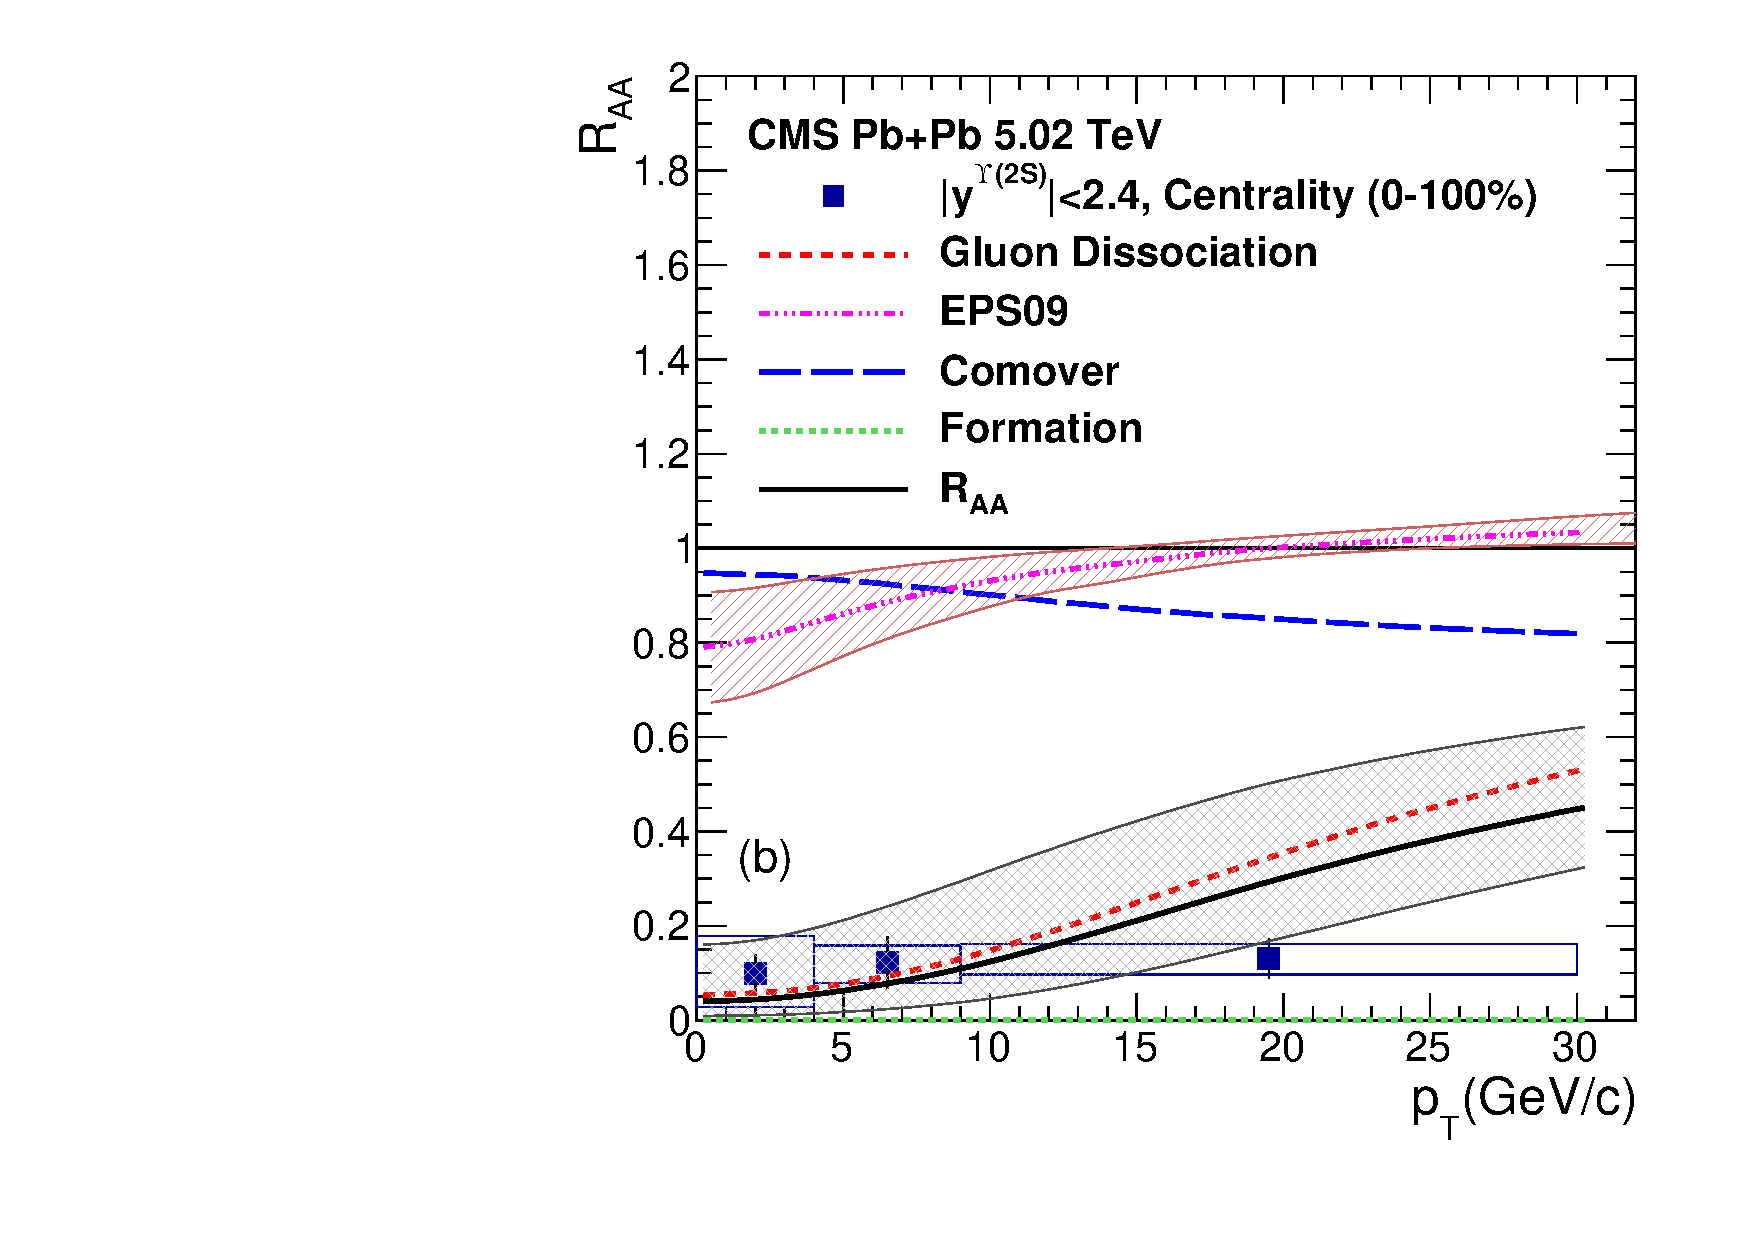
\includegraphics[width=0.49\textwidth]{Fig6b_Y2S_CMS_RAAPt_Shade.pdf}
\caption{(Color online) Calculated nuclear modification factor ($R_{AA}$) of (a) $\Upsilon$(1S) and 
  (b) $\Upsilon$(2S) as a function of $p_{T}$ 
  compared with CMS measurements~\cite{CMS:2017ucd}.}
\label{fig:UpsilonRaaPtCMS}
\end{figure}



\begin{figure}
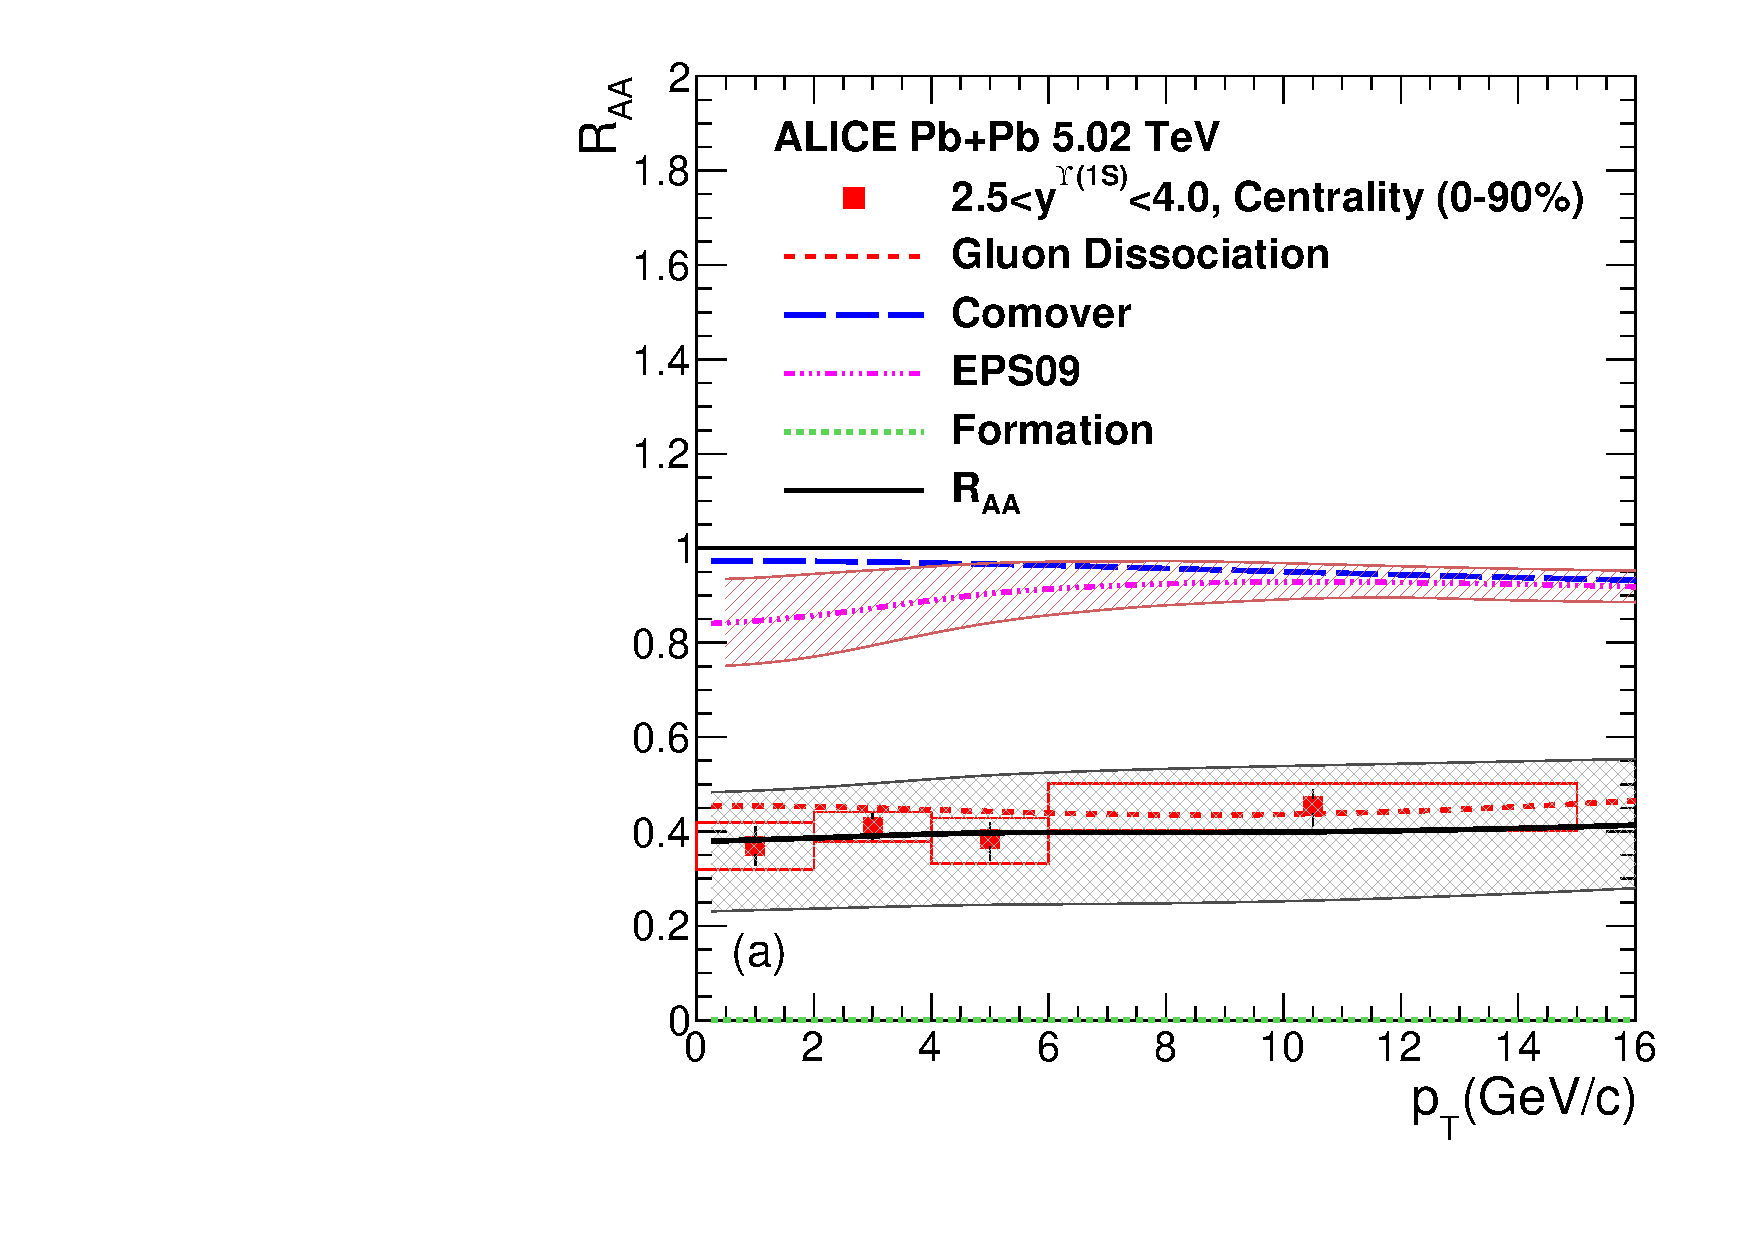
\includegraphics[width=0.49\textwidth]{Fig7a_ALICE_Y1SRAAPt_Shade.pdf}
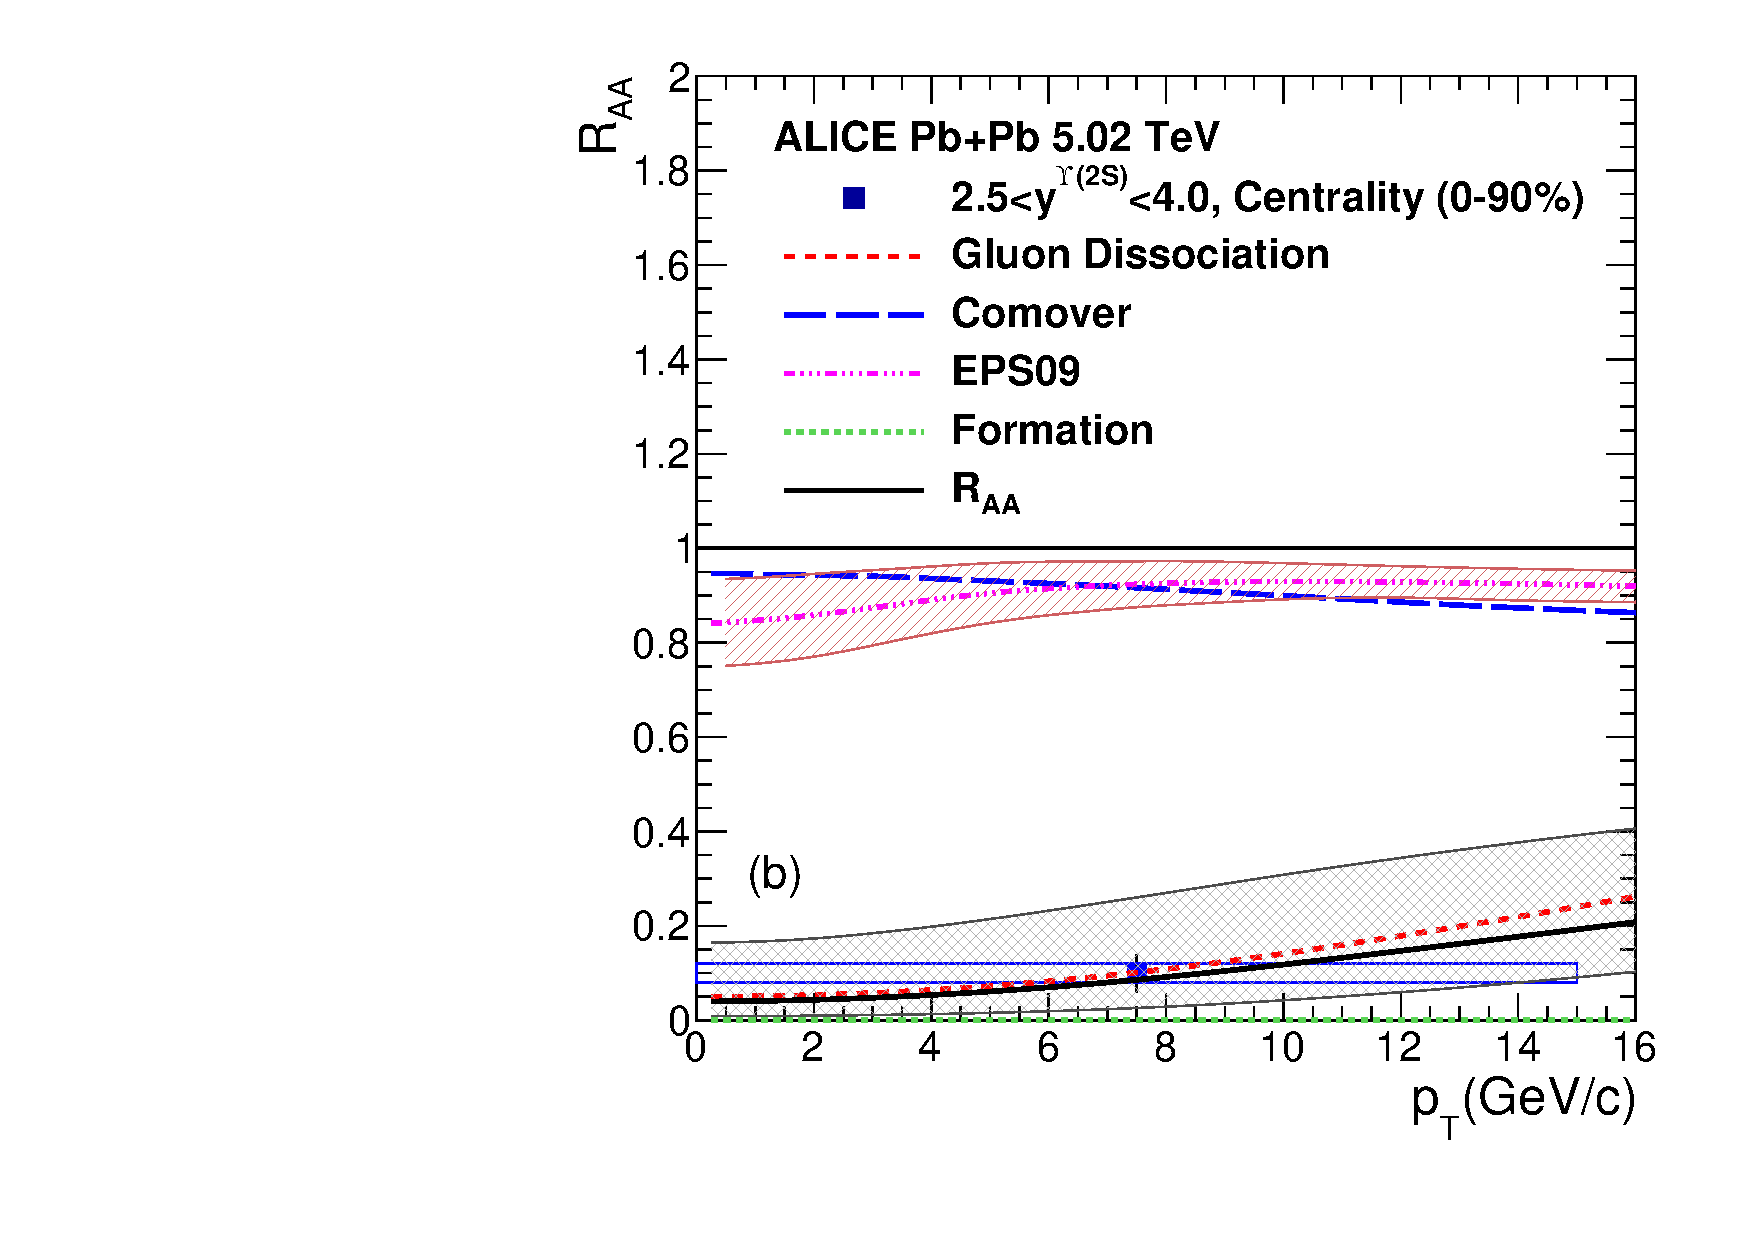
\includegraphics[width=0.49\textwidth]{Fig7b_ALICE_Y2SRAAPt_Shade.pdf}
\caption{(Color online) Calculated nuclear modification factor ($R_{AA}$) of (a) $\Upsilon$(1S) and 
  (b) $\Upsilon$(2S) as a function of $p_{T}$ in the kinetic range of ALICE detector at LHC ~\cite{ALICE:Y5TeV}.} 
 % The calculations are done for the most centreal 0-20$\%$ collisions
  
\label{fig:UpsilonRaaPtALICE}
\end{figure}



\begin{figure}
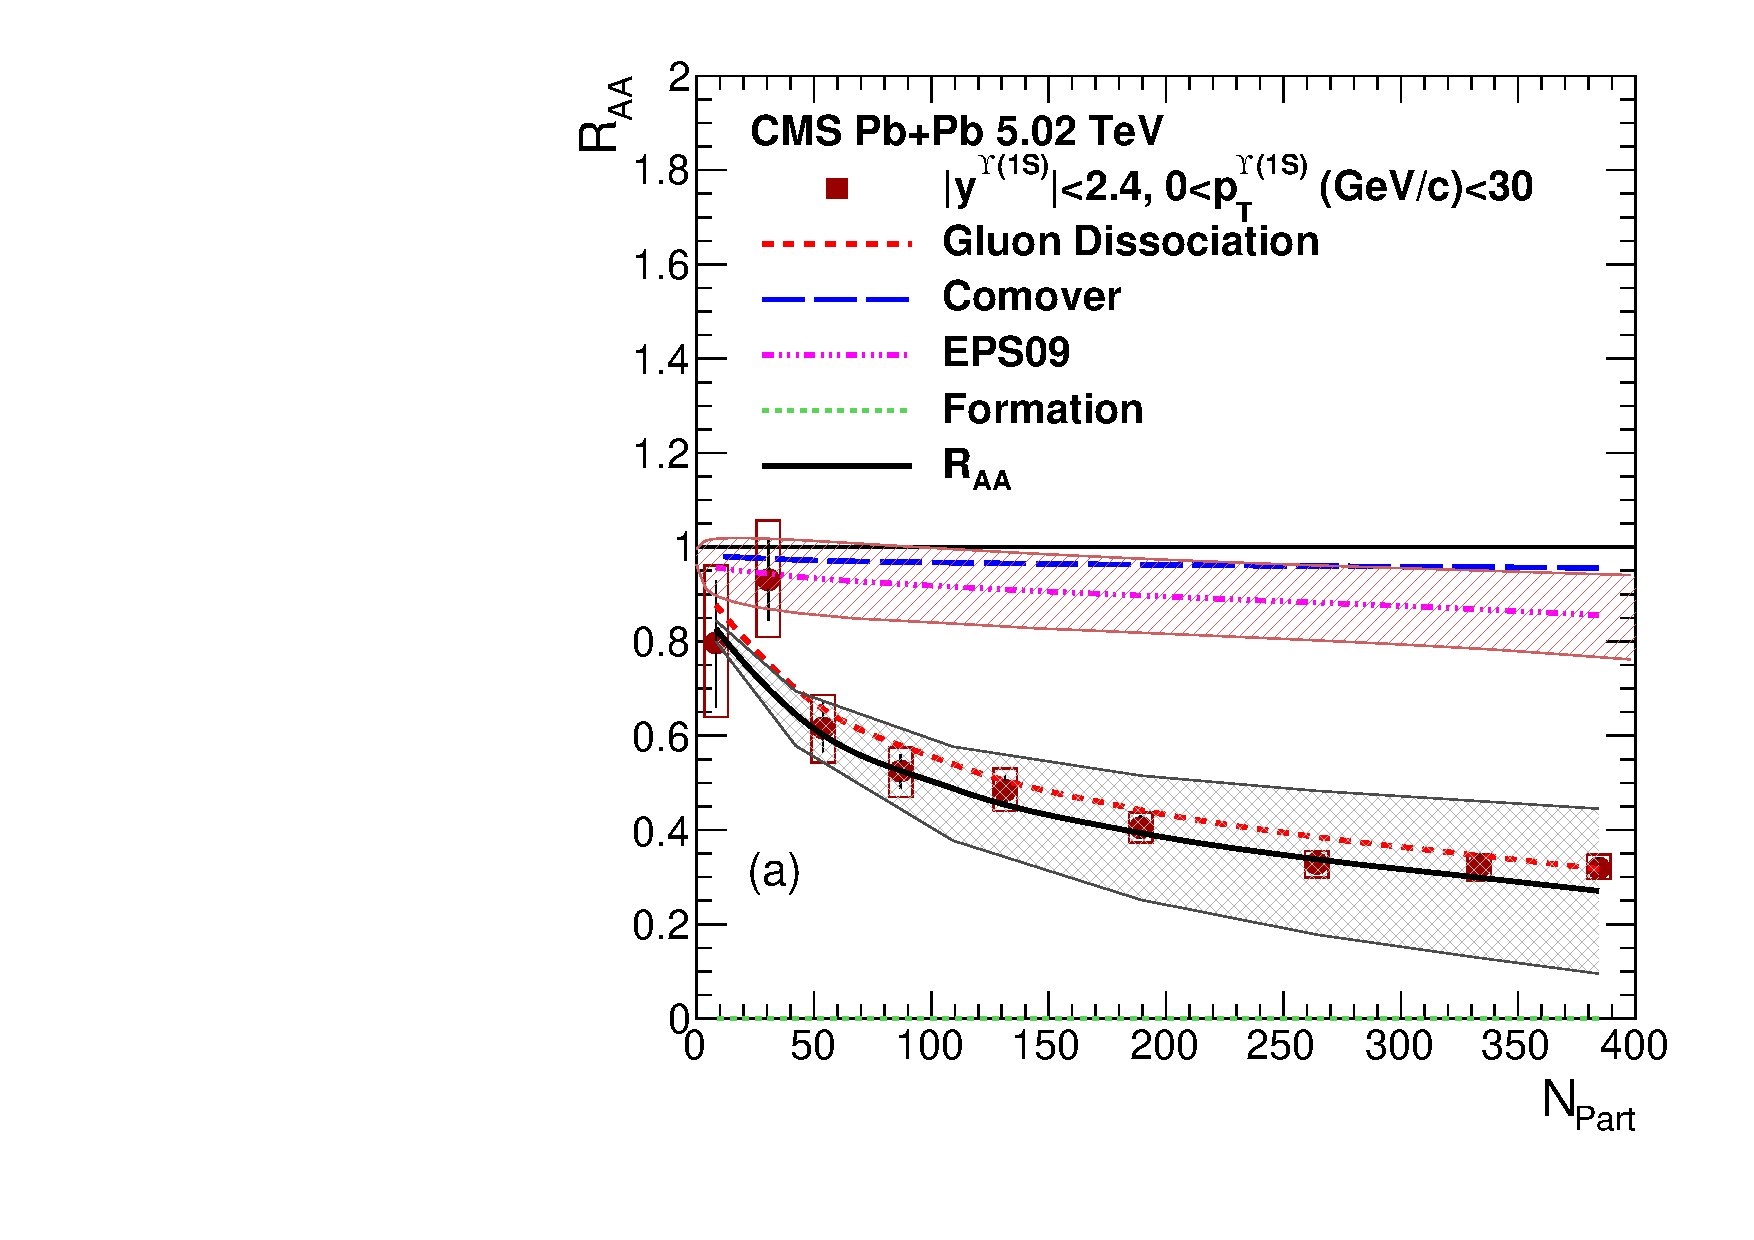
\includegraphics[width=0.49\textwidth]{Fig8a_CMS_Y1SRAANPart_Shade.pdf}
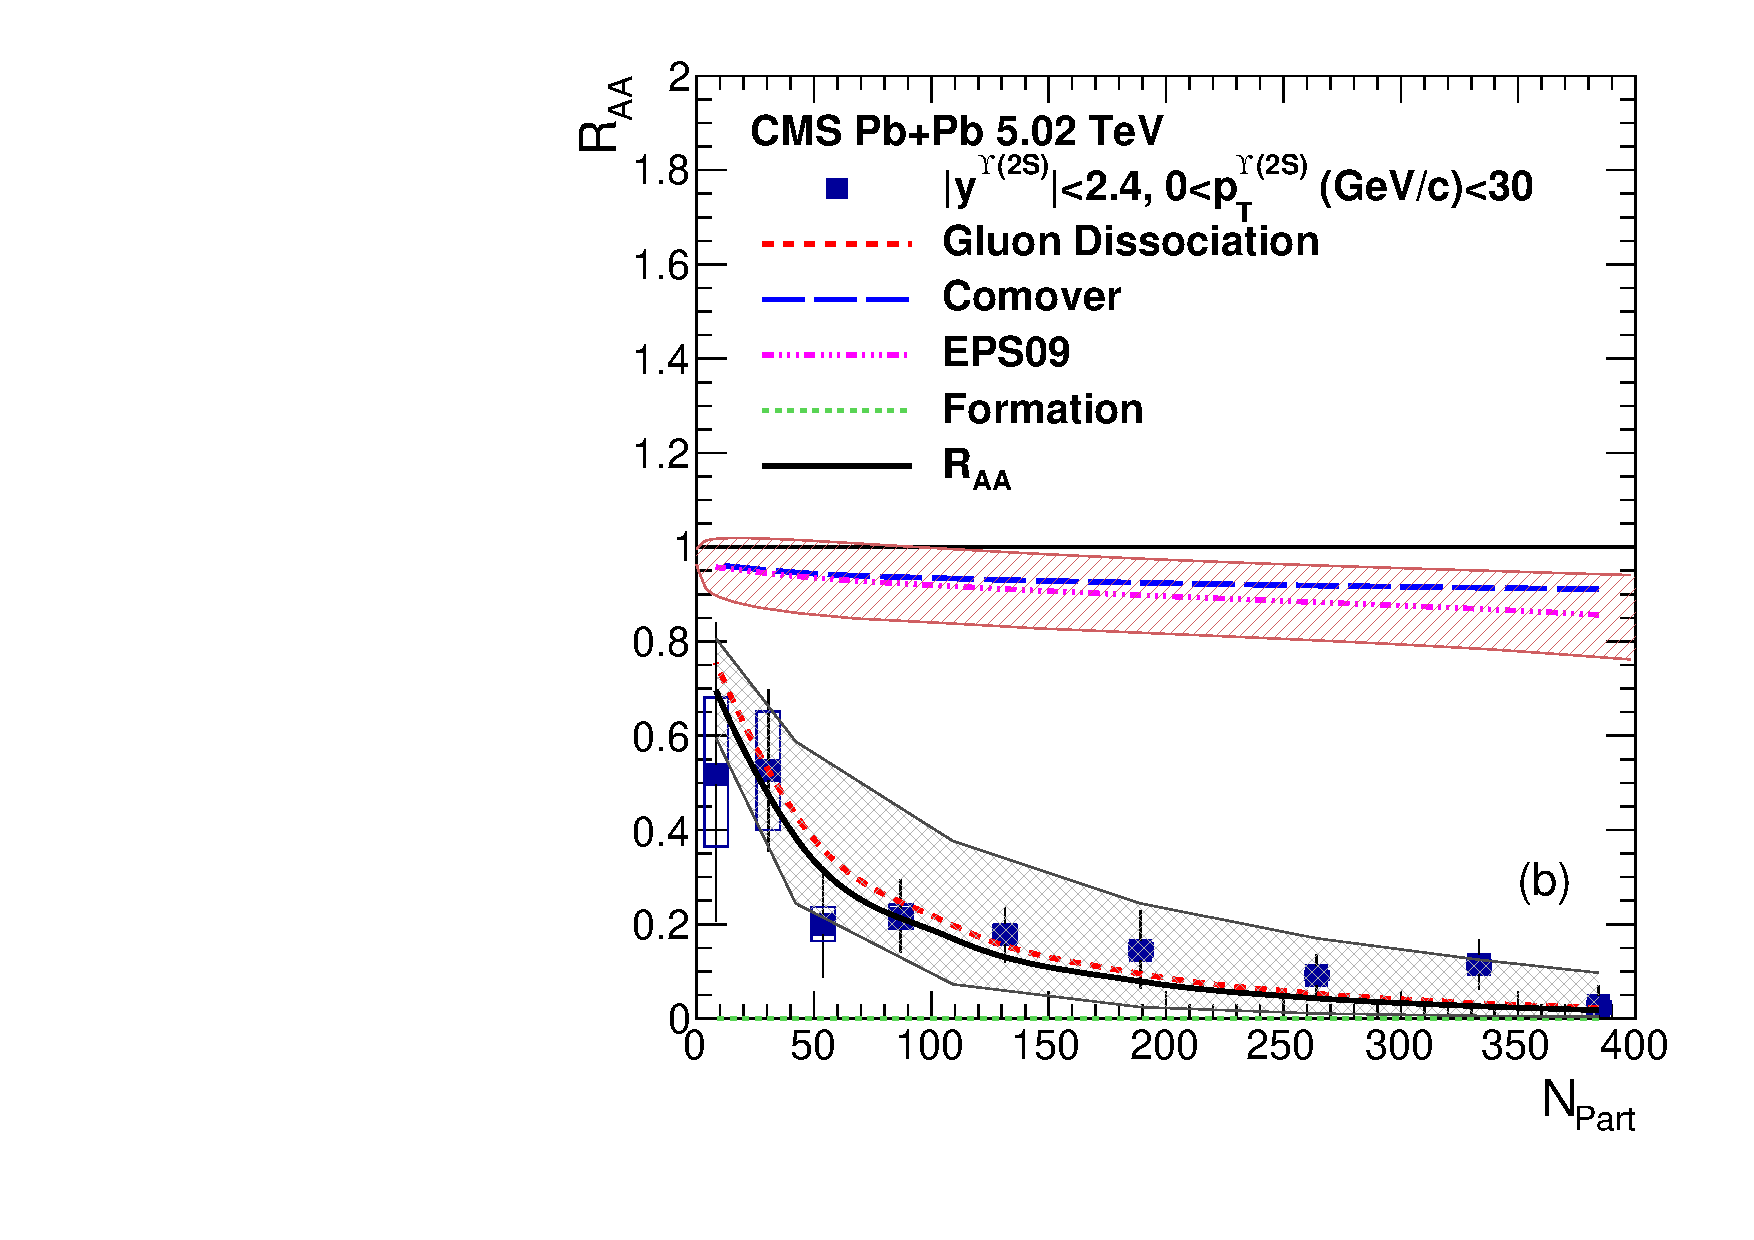
\includegraphics[width=0.49\textwidth]{Fig8b_CMS_Y2SRAANPart_Shade.pdf}
\caption{(Color online) Calculated nuclear modification factor ($R_{AA}$) of 
  (a) $\Upsilon$(1S) and (b) $\Upsilon$(2S) as a function of centrality of the 
  collisions compared with the CMS measurements~\cite{CMS:2017ucd}.}
\label{fig:UpsilonRaaNPartCMS}
\end{figure}


Figure~\ref{fig:JPsiRaaVsPt} (a) and (b) show the estimations of different contributions
to the nuclear modification factor, $R_{AA}$, for the J/$\psi$ meson as a function of $p_T$ 
along with the mid rapidity and high $p_T$ measurements from
CMS~\cite{Sirunyan:2017isk} and ATLAS~\cite{ATLAS:2016qpn} experiments respectively.
Figure~\ref{fig:JPsiRaaVsPt}(c) shows the same for the low $p_T$ and forward
rapidity compared with the measurement by ALICE experiment~\cite{Adam:2016rdg}.
At low $p_T$, regeneration of J/$\psi$ gives dominant
contribution which overcomes the strong suppression by gluon dissociation.
This looks to be the reason for the increase of J/$\psi$ $R_{AA}$ around $p_T\approx$ 2 GeV/c. 
The suppression due to gluon dissociation is substantial at low $p_T$ and reduces as
we move to higher $p_T$. At low and intermediate $p_T$, both regeneration and dissociation, due
to the presence of QGP are effective.  The high $p_T$
suppression ($p_T > 10$  GeV/$c$) of $\Jpsi$ measured by CMS is greater than the
suppression caused by gluon dissociation in the QGP. The suppression measured
by CMS and ATLAS at high $p_T$ values greater than the heavy quark mass,
and thus here the energy loss from initial partonic scatterings might play a
crucial role as it does for open heavy flavour. 

The values of gluon-quarkonia cross section ($\sigma_{D}$) and the initial temperature $T_{0}$
can have uncertainites and will affect the results.
The value of $\sigma_D$ is varied by $\pm$50\% around the calculated value to obtain
the uncertainty in $R_{AA}$.  The initial temperature is calculated using measured
charged particle density and nominal value of $\tau_0 =$ 0.3 fm/$c$. The value of $\tau_0$
is varied  in the range 0.1 $<\,\tau_0\,<$ 0.6 fm/$c$ which corresponds to the
variation in the initial temperature from +45 \% to - 20 \%. The total uncertainty is
obtained by adding in quadrature the above two uncertainties.
The CNM effects are not dominant and hence this uncertainty  is not included in the
total $R_{AA}$ uncertainty band.


 The calculation of $R_{AA}$ of J/$\psi$ is also made as a function of collision
centrality (system size). 
Figure~\ref{fig:JPsiRaaVsNPart} shows calculations of different contributions to the J/$\psi$ 
nuclear modification factor as a function of system size, along with the measurements
from CMS in (a), ATLAS in (b) and ALICE in (c)~\cite{Sirunyan:2017isk,ATLAS:2016qpn,Adam:2016rdg}.
The figure shows that the suppression of J/$\psi$ due to
QGP increases when the system size grows. The contribution from regeneration process
is minimum in the high $p_T$ range ($p_T~>9$ GeV/c) for ATLAS case
as shown in Fig.~\ref{fig:JPsiRaaVsNPart}(b) and maximum in the low $p_T$ range
for the ALICE case shown in Fig.~\ref{fig:JPsiRaaVsNPart}(c). For low $p_T$ ALICE measurement,
the nuclear modification factor is almost flat from mid to central collisions because
the regeneration compensates the gluon dissociation, a trend which is well-reproduced
by our calculations.
The CMS centrality dependence of the $R_{AA}$ of $\Jpsi$ given in
Fig.~\ref{fig:JPsiRaaVsNPart}(a) is reasonably well described by the model since 
the contribution of the CMS data comes from $\Jpsi$ with 6.5 $<\,p_T<\,$10 GeV/$c$
where the suppression due to gluon dissociation dominates.
For the case of ATLAS data, the model reproduces the shape of centrality dependence
of the $R_{AA}$ of $\Jpsi$ observed in the data.
 


\begin{figure}
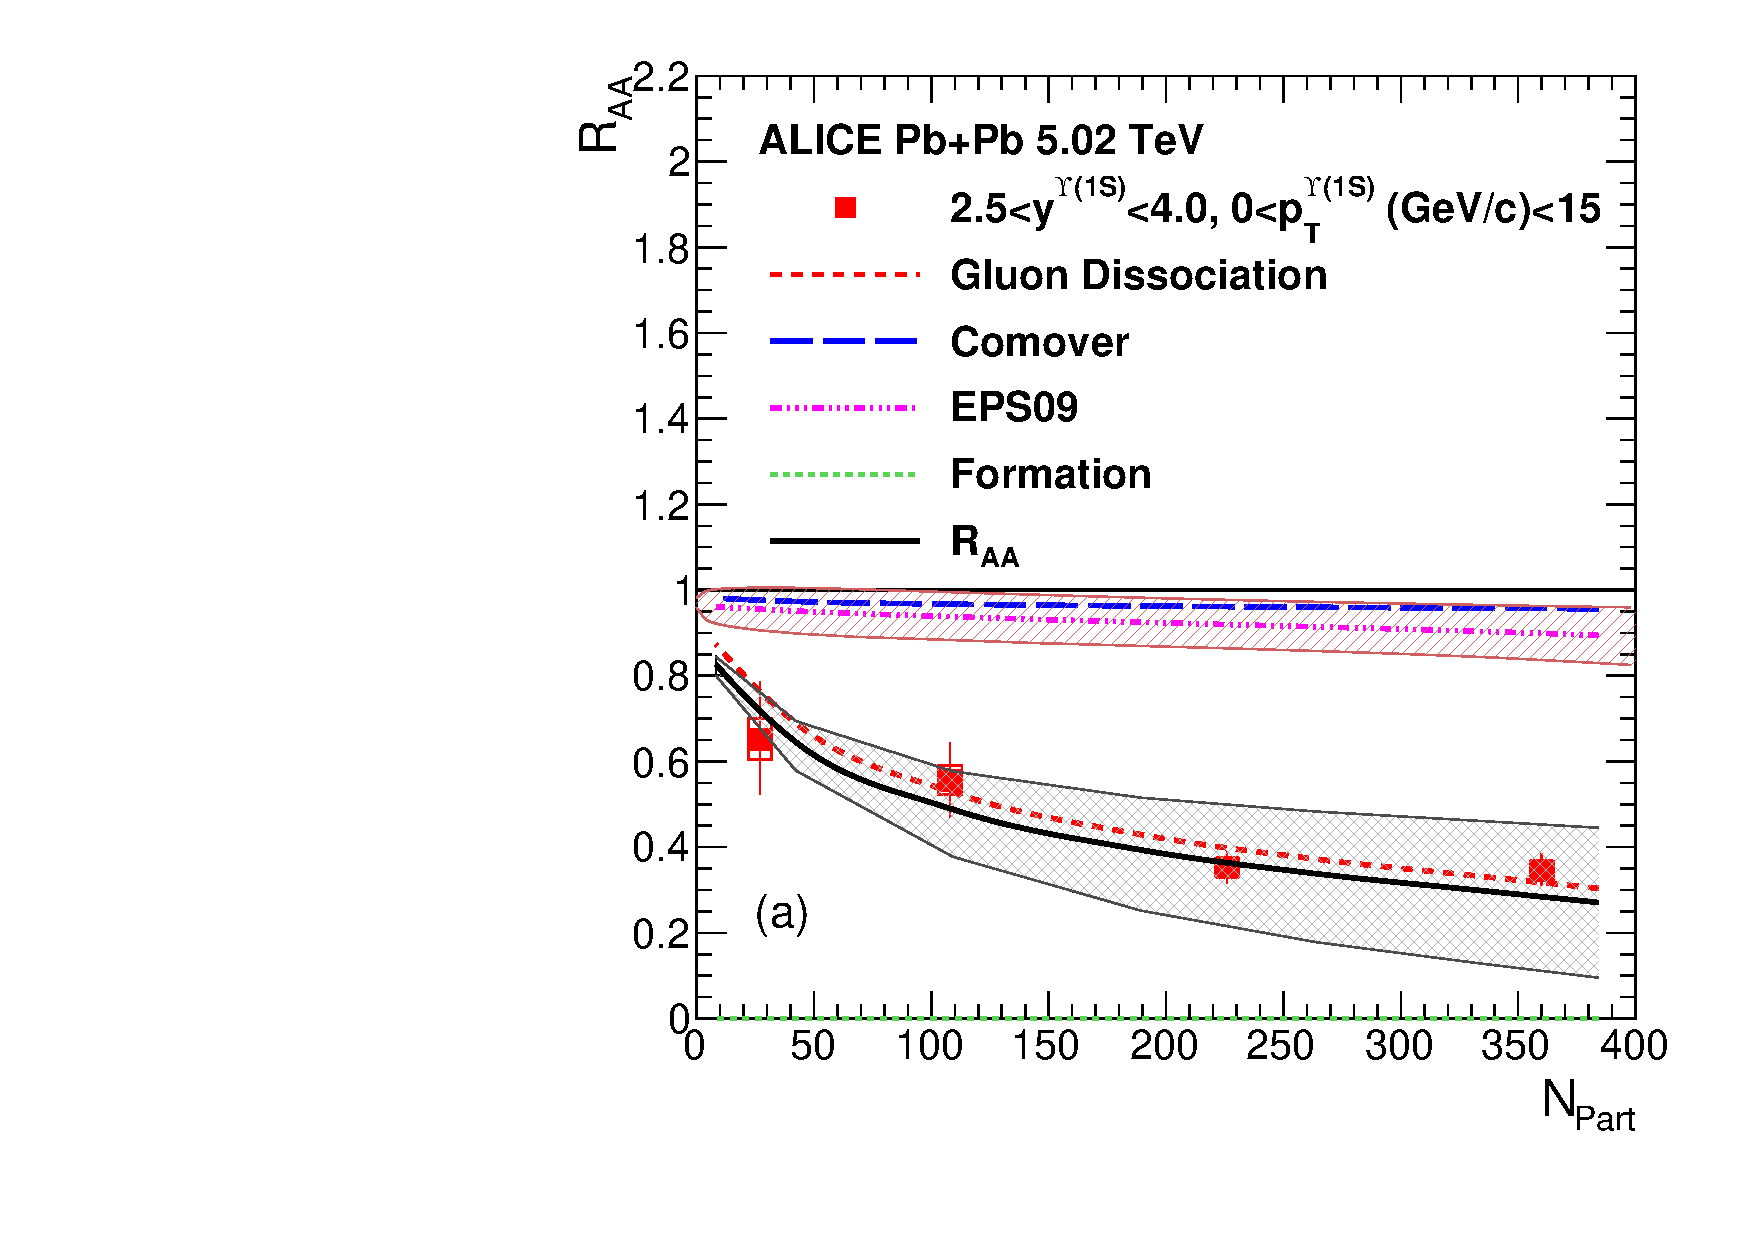
\includegraphics[width=0.49\textwidth]{Fig9a_Y1S_ALICE_RAANPart_Shade.pdf}
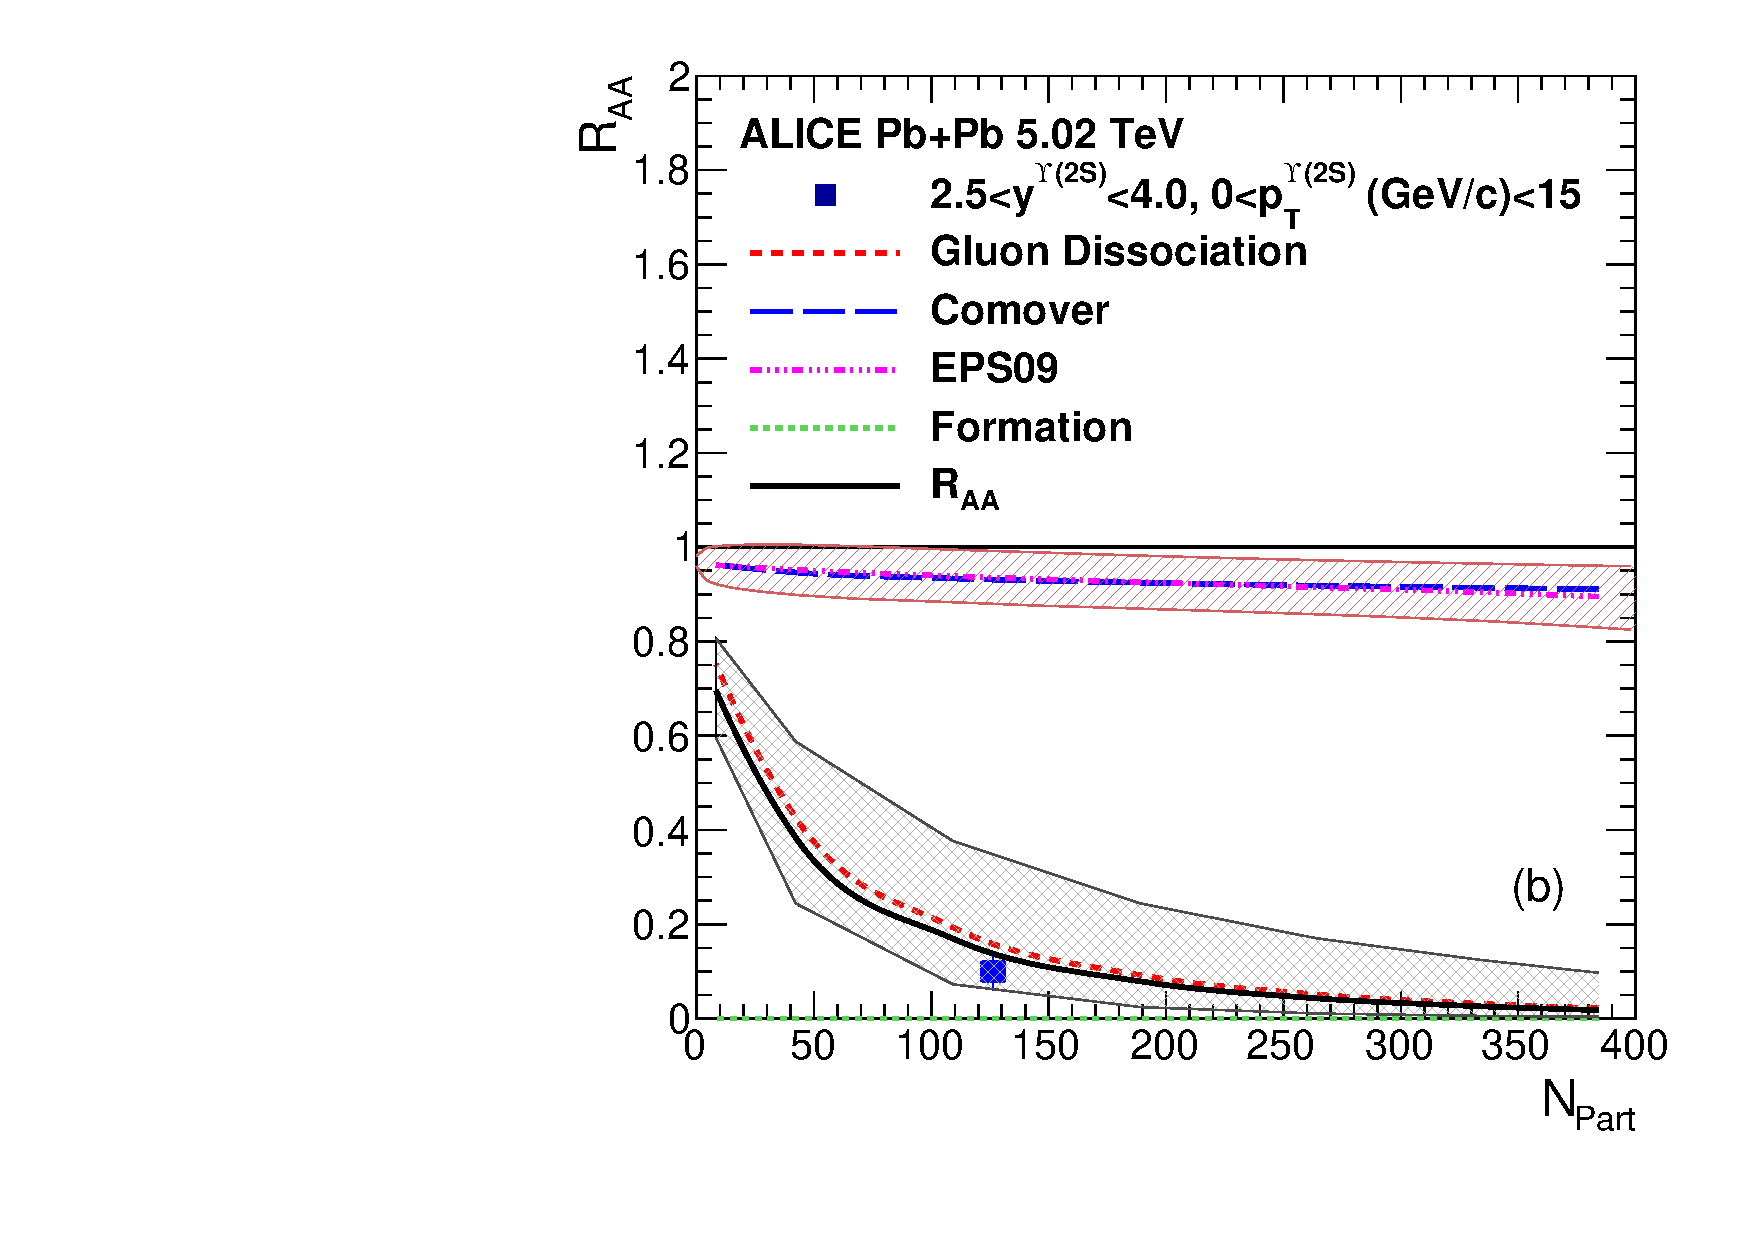
\includegraphics[width=0.49\textwidth]{Fig9b_Y2S_ALICE_RAANPart_Shade.pdf}
\caption{(Color online) Calculated nuclear modification factor ($R_{AA}$) of 
  (a) $\Upsilon$(1S) and (b) $\Upsilon$(2S) as a function of centrality of 
  the collisions compared with the ALICE measurement~\cite{ALICE:Y5TeV}.}
\label{fig:UpsilonRaaNPartALICE}
\end{figure}

Figure~\ref{fig:UpsilonRaaPtCMS} (a) and (b) show the calculations of contributions to
the nuclear modification factor, $R_{AA}$, for the $\Upsilon$(1S) and $\Upsilon$(2S)
respectively as a function of $p_T$ compared with the mid rapidity measurements from
CMS~\cite{CMS:2017ucd}.  
The gluon dissociation mechanism combined with the pion dissociation and shadowing
corrections gives good description of data in mid $p_{T}$ range ($p_{T}\approx$ 5-10 GeV/c)
for both $\Upsilon$(1S) and $\Upsilon$(2S).
The contribution from the regenerated $\Upsilon$s is negligible even at LHC energies.
Our calculations under-predict the suppression observed at the highest measured
$p_{T}$ for $\Upsilon$(1S) and $\Upsilon$(2S) which is similar for the case
of J/$\psi$.
%The feed-down corrections are applied in our calculations following the similar
%procedure as in Refs.~\cite{Abdulsalam:2012bw,Krouppa:2017jlg}. 
%%%%%%%%% insert the feed-down details here
The states $\Upsilon$(1S) and $\Upsilon$(2S) also have
feed-down contributions from decays of higher b$\bar{\rm b}$ bound states.
The nuclear modification factor, $R_{AA}$ is obtained taking into account the feed-down corrections as follows
  \begin{equation}
    R_{AA}^{\Upsilon(3S)} = R_{AA}^{\Upsilon(3S)}\\ %\nonumber
  \end{equation}
  \begin{equation}
    R_{AA}^{\Upsilon(2S)} = f_1 R_{AA}^{\Upsilon(2S)} +  f_2 R_{AA}^{\Upsilon(3S)} \\ %\nonumber
  \end{equation}
   \begin{equation}
    R_{AA}^{\Upsilon(1S)} = g_1 R_{AA}^{\Upsilon(1S)} +  g_2 R_{AA}^{\chi_b(1P)} + g_3 R_{AA}^{\Upsilon(2S)} + g_4 R_{AA}^{\Upsilon(3S)}\\ %\nonumber
  \end{equation}
The factors $f$’s and $g$’s are obtained from CDF measurement~\cite{Affolder:1999wm}.
The values of $g_1$, $g_2$, $g_3$ and $g_4$ are 0.509, 0.27, 0.107
and 0.113 respectively. Here $g_4$ is assumed to be the combined fraction of 
$\Upsilon$(3S) and $\chi_b$(2P).
The values of $f_1$ and $f_2$ are taken as 0.50~\cite{Strickland:2011aa}.


Figure~\ref{fig:UpsilonRaaPtALICE} (a) and (b) show the model 
prediction of the nuclear modification factor, $R_{AA}$, for the $\Upsilon$(1S)
and $\Upsilon$(2S) respectively as a function of $p_T$ in the kinematic range
covered by ALICE detector. The ALICE data~\cite{ALICE:Y5TeV} is well described by our model.

Figure~\ref{fig:UpsilonRaaNPartCMS}(a) depicts the calculated 
centrality dependence of the $\Upsilon$(1S) nuclear
modification factor, along with the midrapidity data from CMS~\cite{CMS:2017ucd}.
Our calculations combined with the pion dissociation and shadowing corrections 
gives very good description of the measured data. Figure~\ref{fig:UpsilonRaaNPartCMS} (b)
shows the same for the $\Upsilon$(2S) along with the midrapidity
CMS measurements. The suppression of the excited $\Upsilon$(2S) states 
is also well described by our model. As stated earlier, the effect of regeneration is
negligible for $\Upsilon$ states. 

Figure~\ref{fig:UpsilonRaaNPartALICE}(a) shows the forward rapidity ALICE
measurement of the $\Upsilon$(1S) nuclear modification factor~\cite{ALICE:Y5TeV}
along with our calculations. The suppression due to thermal gluon dissociation 
describes the measured data after including the comover and shadowing corrections.
Figure~\ref{fig:UpsilonRaaNPartALICE}(b) shows the calculations for the
$\Upsilon$(2S) nuclear modification factor in ALICE detector kinematic range.
The suppression due to thermal gluon dissociation describes the
ALICE measurements after including the comover and shadowing corrections.


%%%%%%%%%%%%%%%%%%%%%%%%%%%%%%%%%%%%%%%%%%%%%%%%%%%%%%%%%%%%%%%%%%%%%%%%%%%%%%%%%%%%%%%
\section{Summary}
 We presented detailed calculations of the $\Jpsi$ and $\Upsilon$ 
production and the modifications their yields in PbPb collisions at $\sNN =$ = 5.02 TeV.
A kinetic model is employed which incorporates quarkonia suppression inside QGP, suppression 
due to hadronic comovers and regeneration from heavy quark pairs.
The behaviour of the dissociation and formation rates are studied as a function of
transverse momentum and medium temperature. 
The nuclear modification factors for both $\Jpsi$ and $\Upsilon$ are obtained 
as a function of system size and transverse momentum and have been compared to the measurements
in PbPb collisions at $\sNN =$ = 5.02 TeV.
It is found that  regeneration of $\Jpsi$ is the dominant process at low $p_T$. As a result the $\Jpsi$ production 
is found to be enhanced in the ALICE low $p_T$ data.
In the same $p_T$ range gluon dissociation is also substantial however it becomes small
as we move to high $p_T$. 
 Both  these processes affect the 
yields of quarkonia in a QGP medium  at low and intermediate $p_T$. The high $p_T$ 
suppression ($p_T > 10$  GeV/$c$) of $\Jpsi$ measured by CMS and ATLAS is more than
the suppression expected due to gluon dissociation in QGP.
As the system size grows  $\Jpsi$'s are increasingly suppressed.  The nuclear 
modification factor at low $p_T$  (ALICE case) as a function of centrality remains
flat since the increased suppression is compensated by regenerated  $\Jpsi$'s
as the system size grows. 
We could reproduce the centrality dependence of $R_{AA}$ for high $p_T$ $\Jpsi$'s reasonably
well. 
 The $\pT$ and centrality dependence of suppression of $\Upsilon$ states are well reproduced
by the model.
 
\section{Acknowledgement}
Authors thank Board of Research in Nuclear Sciences (BRNS) and Alexander von Humboldt (AvH)
foundation for support. 

%\bibliographystyle{plain}
%\bibliography{upsilon}

\section*{References}
%\noindent
\begin{thebibliography}{100}
%\medskip

\bibitem{Busza:2018rrf} 
  W.~Busza, K.~Rajagopal and W.~van der Schee,
  ``Heavy Ion Collisions: The Big Picture, and the Big Questions,''
  arXiv:1802.04801 [hep-ph].
  

 
\bibitem{Shuryak:2017aol} 
  E.~Shuryak,
  ``The sounds of the Little and Big Bangs,''
  Universe {\bf 3}, 75 (2017),
  [arXiv:1710.03776 [hep-ph]].
  

\bibitem{Brambilla:2010cs} 
  N.~Brambilla, S.~Eidelman, B.~K.~Heltsley, R.~Vogt, G.~T.~Bodwin, E.~Eichten, A.~D.~Frawley and A.~B.~Meyer {\it et al.},
  ``Heavy quarkonium: progress, puzzles, and opportunities,''
  Eur.\ Phys.\ J.\ C {\bf 71}, 1534 (2011).
  %[arXiv:1010.5827 [hep-ph]].


\bibitem{Matsui:1986dk} 
 T.~Matsui and H.~Satz,
 ``J/$\psi$ Suppression by Quark-Gluon Plasma Formation'',
 Phys.\ Lett.\ B {\bf 178}, 416 (1986).

\bibitem{Hashimoto:1986nn} 
  T.~Hashimoto, K.~Hirose, T.~Kanki and O.~Miyamura,
  ``Mass Shift of Charmonium Near Deconfining Temperature and Possible Detection in Lepton Pair Production,''
  Phys.\ Rev.\ Lett.\  {\bf 57}, 2123 (1986).



\bibitem{Schukraft:2013wba} 
  J.~Schukraft,
  ``Heavy ion physics at the Large Hadron Collider: what is new? What is next?,''
  Phys.\ Scripta T {\bf 158}, 014003 (2013), [arXiv:1311.1429 [hep-ex]].
  

\bibitem{Andronic:2015wma} 
  A.~Andronic {\it et al.},
  ``Heavy-flavour and quarkonium production in the LHC era: from proton–proton to heavy-ion collisions,''
  Eur.\ Phys.\ J.\ C {\bf 76}, 107 (2016), [arXiv:1506.03981 [nucl-ex]].


\bibitem{Alessandro:2004ap} 
  B.~Alessandro {\it et al.} [NA50 Collaboration],
  ``A New measurement of J/$\psi$ suppression in PbPb collisions at 158-GeV per nucleon,''
  Eur.\ Phys.\ J.\ C {\bf 39}, 335 (2005), [hep-ex/0412036].
 
\bibitem{Arnaldi:2007zz} 
  R.~Arnaldi {\it et al.} [NA60 Collaboration],
  ``J/$\psi$ production in indium-indium collisions at 158-GeV/nucleon,''
  Phys.\ Rev.\ Lett.\ {\bf 99}, 132302 (2007).
  

\bibitem{Adare:2011yf} 
A.~Adare {\it et al.}  [PHENIX Collaboration],
  ``J/$\psi$ suppression at forward rapidity in AuAu collisions at $\sqrt{s_{NN}}$ = 200 GeV,''
  Phys.\ Rev.\ C {\bf 84}, 054912 (2011), [arXiv:1103.6269 [nucl-ex]].

\bibitem{Abelev:2009qaa} 
  B.~I.~Abelev {\it et al.} [STAR Collaboration],
  ``J/$\psi$ production at high transverse momentum in pp and CuCu collisions at  $\sqrt{s_{NN}}$ = 200 GeV,''
  Phys.\ Rev.\ C {\bf 80}, 041902 (2009), [arXiv:0904.0439 [nucl-ex]].

\bibitem{Tang:2011kr} 
  Z.~Tang [STAR Collaboration],
  ``J/$\psi$ production and correlation in pp and AuAu collisions at STAR,''
  J.\ Phys.\ G {\bf 38}, 124107 (2011).
 %[arXiv:1107.0532 [hep-ex]].

  
\bibitem{Aad:2010aa} 
  G.~Aad {\it et al.} [ATLAS Collaboration],
  ``Measurement of the centrality dependence of $\Jpsi$ yields and observation of Z production in 
  lead–lead collisions with the ATLAS detector at the LHC,''
  Phys.\ Lett.\ B {\bf 697}, 294 (2011), [arXiv:1012.5419 [hep-ex]].


%\bibitem{Muller:2012zq} 
%  B.~Muller, J.~Schukraft and B.~Wyslouch,
%  ``First Results from PbPb collisions at the LHC,''
%  Ann.\ Rev.\ Nucl.\ Part.\ Sci.\  {\bf 62}, 361 (2012).
%%  [arXiv:1202.3233 [hep-ex]].


\bibitem{Chatrchyan:2012np} 
  S.~Chatrchyan {\it et al.}  [CMS Collaboration],
  ``Suppression of non-prompt J/$\psi$, prompt J/$\psi$, and $\Upsilon$(1S) in PbPb collisions at $\sqrt{s_{NN}}=2.76$ TeV,''
  JHEP {\bf 1205}, 063 (2012), [arXiv:1201.5069 [nucl-ex]].

\bibitem{Khachatryan:2016ypw} 
  V.~Khachatryan {\it et al.} [CMS Collaboration],
  ``Suppression and azimuthal anisotropy of prompt and nonprompt ${\mathrm{J}}/\psi $ production in PbPb collisions at $\sqrt{{s_{_{{\rm NN}}}}} =2.76$ $\,\mathrm{TeV}$,'' Eur.\ Phys.\ J.\ C {\bf 77}, 252 (2017)
  [arXiv:1610.00613 [nucl-ex]].


%\bibitem{Sirunyan:2017isk} 
%  A.~M.~Sirunyan {\it et al.} [CMS Collaboration],
%  ``Measurement of prompt and nonprompt charmonium suppression in PbPb collisions at 5.02 TeV,''
%  arXiv:1712.08959 [nucl-ex].



\bibitem{Sirunyan:2017isk} 
  A.~M.~Sirunyan {\it et al.} [CMS Collaboration],
  ``Measurement of prompt and nonprompt charmonium suppression in PbPb collisions at 5.02 TeV,''
  Eur.\ Phys.\ J.\ C {\bf 78}, no. 6, 509 (2018),
  [arXiv:1712.08959 [nucl-ex]].
  %%CITATION = doi:10.1140/epjc/s10052-018-5950-6;%%
  %11 citations counted in INSPIRE as of 27 Sep 2018



\bibitem{ATLAS:2016qpn} 
  The ATLAS collaboration [ATLAS Collaboration],
  ``Study of J/$\psi\to\mu^+\mu^-$ and $\psi\mathrm{(2S)}\to\mu^+\mu^-$ production with 2015 PbPb data at 
  $\sqrt{s_{\mathrm{NN}}} = 5.02~\mathrm {TeV}$ and pp data at $\sqrt{s} = 5.02~\mathrm {TeV}$ with the 
  ATLAS detector,'' ATLAS-CONF-2016-109.

\bibitem{Abelev:2013ila} 
  B.~B.~Abelev {\it et al.}  [ALICE Collaboration],
  ``Centrality, rapidity and transverse momentum dependence of J/$\psi$ suppression in PbPb collisions at $\sqrt{s_{NN}}$=2.76 TeV,''
  Phys.\ Lett.\  {\bf 743}, 314 (2014), [arXiv:1311.0214 [nucl-ex]].


\bibitem{Adam:2016rdg} 
  J.~Adam {\it et al.} [ALICE Collaboration],
  ``J/$\psi$ suppression at forward rapidity in PbPb collisions at $\mathbf{\sqrt{s_{{\rm NN}}} = 5.02}$ TeV,''
  Phys.\ Lett.\ B {\bf 766}, 212 (2017), [arXiv:1606.08197 [nucl-ex]].


\bibitem{Acharya:2017tgv} 
  S.~Acharya {\it et al.} [ALICE Collaboration],
  ``J/$\psi$ elliptic flow in PbPb collisions at $\sqrt{s_\mathrm{NN}}=5.02$ TeV,''
  Phys.\ Rev.\ Lett.\  {\bf 119}, 242301 (2017),
  [arXiv:1709.05260 [nucl-ex]].


\bibitem{Digal:2001ue} 
  S.~Digal, P.~Petreczky and H.~Satz,
  ``Quarkonium feed down and sequential suppression,''
  Phys.\ Rev.\ D {\bf 64}, 094015 (2001), [hep-ph/0106017].

\bibitem{Andronic:2003zv} 
  A.~Andronic, P.~Braun-Munzinger, K.~Redlich and J.~Stachel,
  ``Statistical hadronization of charm in heavy ion collisions at SPS, RHIC and LHC,''
  Phys.\ Lett.\ B {\bf 571}, 36 (2003).
 % [nucl-th/0303036].


\bibitem{Thews:2000rj} 
  R.~L.~Thews, M.~Schroedter and J.~Rafelski,
  ``Enhanced J/$\psi$ production in deconfined quark matter,''
  Phys.\ Rev.\ C {\bf 63}, 054905 (2001).
  %[hep-ph/0007323].



\bibitem{Du:2017qkv} 
  X.~Du, R.~Rapp and M.~He,
  ``Color Screening and Regeneration of Bottomonia in High-Energy Heavy-Ion Collisions,''
  Phys.\ Rev.\ C {\bf 96}, 054901 (2017), [arXiv:1706.08670 [hep-ph]].






  
\bibitem{P.ShuklaforCMS:2014vna} 
  P.~Shukla [CMS Collaboration],
  %``Overview of quarkonia and heavy flavour measurements by CMS,''
  Proc.\ Indian Natl.\ Sci.\ Acad.\  {\bf 81}, 199 (2015).
  [arXiv:1405.3810 [nucl-ex]].


\bibitem{Kumar:2014kfa} 
  V.~Kumar, P.~Shukla and R.~Vogt,
  ``Quarkonia suppression in PbPb collisions at $\sqrt{s_{NN}}$ = 2.76 TeV,''
  Phys.\ Rev.\ C {\bf 92}, 024908 (2015),
  [arXiv:1410.3299 [hep-ph]].



\bibitem{Chatrchyan:2011pe} 
  S.~Chatrchyan {\it et al.}  [CMS Collaboration],
  ``Indications of suppression of excited $\Upsilon$ states in PbPb collisions at $\sqrt{S_{NN}}$ = 2.76 TeV,''
 Phys.\ Rev.\ Lett.\  {\bf 107}, 052302 (2011).
  %[arXiv:1105.4894 [nucl-ex]].

\bibitem{Chatrchyan:2012lxa} 
  S.~Chatrchyan {\it et al.}  [CMS Collaboration],
  ``Observation of sequential Upsilon suppression in PbPb collisions,''
  Phys.\ Rev.\ Lett.\  {\bf 109}, 222301 (2012).
  %[arXiv:1208.2826 [nucl-ex]].

\bibitem{Abelev:2014nua} 
  B.~B.~Abelev {\it et al.} [ALICE Collaboration],
  ``Suppression of $\Upsilon$(1S) at forward rapidity in PbPb collisions at $\sqrt{s_{\rm NN}} = 2.76$ TeV,''
  Phys.\ Lett.\ B {\bf 738}, 361 (2014), [arXiv:1405.4493 [nucl-ex]].
  
  
\bibitem{Khachatryan:2016xxp} 
  V.~Khachatryan {\it et al.} [CMS Collaboration],
  ``Suppression of $\Upsilon$(1S), $\Upsilon$(2S) and $\Upsilon$(3S) production in PbPb collisions at $\sqrt{s_{\rm NN}}$ = 2.76 TeV,''
  Phys.\ Lett.\ B {\bf 770}, 357 (2017), [arXiv:1611.01510 [nucl-ex]].


\bibitem{Sirunyan:2017lzi} 
  A.~M.~Sirunyan {\it et al.} [CMS Collaboration],
  ``Suppression of Excited $\Upsilon$ States Relative to the Ground State in PbPb Collisions at $\sqrt{s_\mathrm{NN}}$ = 5.02 TeV,''
  Phys.\ Rev.\ Lett.\  {\bf 120}, 142301 (2018), [arXiv:1706.05984 [hep-ex]].
  


\bibitem{CMS:2017ucd} 
  CMS Collaboration [CMS Collaboration],
  ``Measurement of Nuclear Modification Factors of $\Upsilon\textrm{(nS)}$ Mesons in ${\rm PbPb}$ Collisions 
  at $\sqrt{s_{_{{\rm NN}}}} = 5.02~\mathrm{TeV}$,''  CMS-PAS-HIN-16-023.


\bibitem{ALICE:Y5TeV} 
  Antoine Lardeux for [ALICE Collaboration],
   ``$\Upsilon$ production measurements in pPb and Pb–Pb collisions $\sNN =$ 5.02 TeV with ALICE'' SQM2016, UC Berkeley.
 
\bibitem{Karsch:1987pv} 
  F.~Karsch, M.~T.~Mehr and H.~Satz,
  ``Color Screening and Deconfinement for Bound States of Heavy Quarks,''
  Z.\ Phys.\ C {\bf 37}, 617 (1988).

\bibitem{Abdulsalam:2012bw} 
  A.~Abdulsalam and P.~Shukla,
  ``Suppression of bottomonia states in finite size quark gluon plasma in PbPb collisions at Large Hadron Collider,''
  Int.\ J.\ Mod.\ Phys.\ A {\bf 28}, 1350105 (2013).
  %[arXiv:1210.7584 [hep-ph]].

  
\bibitem{Bhanot:1979vb} 
  G.~Bhanot and M.~E.~Peskin,
  ``Short Distance Analysis for Heavy Quark Systems. 2. Applications,''
  Nucl.\ Phys.\ B {\bf 156}, 391 (1979).

\bibitem{Chen:2017jje} 
  S.~Chen and M.~He,
  ``Gluo-dissociation of heavy quarkonium in the quark-gluon plasma reexamined,''
  Phys.\ Rev.\ C {\bf 96}, 034901 (2017),
  [arXiv:1705.10110 [nucl-th]].
  %%CITATION = doi:10.1103/PhysRevC.96.034901;%%

  

%\bibitem{Xu:1995eb} 
%  X.~-M.~Xu, D.~Kharzeev, H.~Satz and X.~-N.~Wang,
%  ``J/$\psi$ suppression in an equilibrating parton plasma,''
%  Phys.\ Rev.\ C {\bf 53}, 3051 (1996).
%  %[hep-ph/9511331].

%\bibitem{Andronic:2012dm} 
%  A.~Andronic, P.~Braun-Munzinger, K.~Redlich and J.~Stachel,
%  ``The statistical model in PbPb collisions at the LHC,''
%  Nucl.\ Phys.\ A {\bf 904-905}, 535c (2013).
%  %[arXiv:1210.7724 [nucl-th]].



%\bibitem{Vogt:2010aa} 
%  R.~Vogt,
%  ``Cold Nuclear Matter Effects on J/$\psi$ and $\Upsilon$ Production at the LHC,''
%  Phys.\ Rev.\ C {\bf 81}, 044903 (2010).
%  %[arXiv:1003.3497 [hep-ph]].


\bibitem{Vogt:2015uba} 
  R.~Vogt,
  ``Shadowing effects on J/$\psi$ and $\Upsilon$ production at energies available at the CERN Large Hadron Collider,''
  Phys.\ Rev.\ C {\bf 92}, 034909 (2015), [arXiv:1507.04418 [hep-ph]].


\bibitem{Ferreiro:2014bia} 
  E.~G.~Ferreiro,
  ``Excited charmonium suppression in proton–nucleus collisions as a consequence of comovers,''
  Phys.\ Lett.\ B {\bf 749}, 98 (2015), [arXiv:1411.0549 [hep-ph]].

%\bibitem{Zhao:2011cv} 
%  X.~Zhao and R.~Rapp,
%  ``Medium Modifications and Production of Charmonia at LHC,''
%  Nucl.\ Phys.\ A {\bf 859}, 114 (2011).
%  %[arXiv:1102.2194 [hep-ph]].

  
\bibitem{Rapp:2017chc} 
  R.~Rapp and X.~Du,
  ``Theoretical Perspective on Quarkonia from SPS via RHIC to LHC,''
  Nucl.\ Phys.\ A {\bf 967}, 216 (2017), [arXiv:1704.07923 [hep-ph]].


\bibitem{Krouppa:2015yoa} 
  B.~Krouppa, R.~Ryblewski and M.~Strickland,
  ``Bottomonia suppression in 2.76 TeV PbPb collisions,'' 
  Phys.\ Rev.\ C {\bf 92}, 061901 (2015),
  [arXiv:1507.03951 [hep-ph]].
  
\bibitem{Krouppa:2017jlg} 
  B.~Krouppa, A.~Rothkopf and M.~Strickland,
  ``Bottomonium suppression using a lattice QCD vetted potential,''
  Phys.\ Rev.\ D {\bf 97}, 016017 (2018), [arXiv:1710.02319 [hep-ph]].



  

%\cite{Oh:2001rm}
\bibitem{Oh:2001rm} 
  Y.~s.~Oh, S.~Kim and S.~H.~Lee,
  ``Quarkonium hadron interactions in QCD,''
  Phys.\ Rev.\ C {\bf 65}, 067901 (2002),
  %doi:10.1103/PhysRevC.65.067901
  [hep-ph/0111132].
  %%CITATION = doi:10.1103/PhysRevC.65.067901;%%
  %58 citations counted in INSPIRE as of 24 Dec 2018

  
\bibitem{Thews:2005vj} 
  R.~L.~Thews and M.~L.~Mangano,
  ``Momentum spectra of charmonium produced in a quark-gluon plasma,''
  Phys.\ Rev.\ C {\bf 73}, 014904 (2006).
  %[nucl-th/0505055].

  
\bibitem{Huovinen:2009yb} 
  P.~Huovinen and P.~Petreczky,
  ``QCD Equation of State and Hadron Resonance Gas,''
  Nucl.\ Phys.\ A {\bf 837}, 26 (2010).
  %[arXiv:0912.2541 [hep-ph]].

\bibitem{Shuryak:1992wc} 
  E.~V.~Shuryak,
  ``Two stage equilibration in high-energy heavy ion collisions,''
  Phys.\ Rev.\ Lett.\  {\bf 68}, 3270 (1992).

\bibitem{Adam:2015ptt} 
  J.~Adam {\it et al.} [ALICE Collaboration],
  ``Centrality dependence of the charged-particle multiplicity density at midrapidity in PbPb collisions at $\sqrt{s_{\rm NN}}$ = 5.02 TeV,''
  Phys.\ Rev.\ Lett.\  {\bf 116}, 222302 (2016),[arXiv:1512.06104 [nucl-ex]].
  
  
\bibitem{Vogt:1988fj} 
  R.~Vogt, M.~Prakash, P.~Koch and T.~H.~Hansson,
  ``J/$\psi$ Interactions With Hot Hadronic Matter,''
  Phys.\ Lett.\ B {\bf 207}, 263 (1988).

\bibitem{Arleo:2001mp} 
  F.~Arleo, P.~B.~Gossiaux, T.~Gousset and J.~Aichelin,
  ``Heavy quarkonium hadron cross section in QCD at leading twist,''
  Phys.\ Rev.\ D {\bf 65}, 014005 (2002).
  %[hep-ph/0102095].

\bibitem{Gluck:1991ey} 
  M.~Glueck, E.~Reya and A.~Vogt,
  ``Pionic parton distributions,''
  Z.\ Phys.\ C {\bf 53}, 651 (1992).

\bibitem{Lourenco:2008sk} 
  C.~Lourenco, R.~Vogt and H.~K.~Woehri,
  ``Energy dependence of J/$\psi$ absorption in proton-nucleus collisions,''
  JHEP {\bf 0902}, 014 (2009).
 %[arXiv:0901.3054 [hep-ph]].










  


%% ========================= pp cross-section reference =============================%%

%%ccbar cross-section ALICE
\bibitem{Abelev:2012vra} 
  B.~Abelev {\it et al.} [ALICE Collaboration],
  ``Measurement of charm production at central rapidity in proton-proton collisions at $\sqrt{s}=2.76$ TeV,''
  JHEP {\bf 1207}, 191 (2012),
  %doi:10.1007/JHEP07(2012)191
  [arXiv:1205.4007 [hep-ex]].
  
%%ccbar cross-section ALICE
\bibitem{Adam:2016ich} 
  J.~Adam {\it et al.} [ALICE Collaboration],
  ``$D$-meson production in $p$Pb collisions at $\sqrt{s_{\rm NN}}=$5.02 TeV and in pp collisions at $\sqrt{s}=$7 TeV,''
  Phys.\ Rev.\ C {\bf 94}, 054908 (2016),
  %doi:10.1103/PhysRevC.94.054908
  [arXiv:1605.07569 [nucl-ex]].
  
%%ccbar cross-section ATLAS
\bibitem{ATLAS:2011fea} 
  [ATLAS Collaboration],
  ``Measurement of D$^(*)$ meson production cross sections in pp collisions at $ \sqrt{s}=7$ TeV with the ATLAS detector,''
  ATLAS-CONF-2011-017.
 
%%ccbar cross-section ATLAS
\bibitem{Aad:2015zix} 
  G.~Aad {\it et al.} [ATLAS Collaboration],
  ``Measurement of $D^{*\pm}$, $D^\pm$ and $D_s^\pm$ meson production cross sections in $pp$ collisions at $\sqrt{s}=7$ TeV with the ATLAS detector,''
  Nucl.\ Phys.\ B {\bf 907}, 717 (2016),
  %doi:10.1016/j.nuclphysb.2016.04.032
  [arXiv:1512.02913 [hep-ex]].
 


%%ccbar cross-section LHCb
\bibitem{LHCb:2010lga} 
  [LHCb Collaboration],
  ``Prompt charm production in $pp$ collisions at $\sqrt{s}$ = 7 TeV,''
  LHCb-CONF-2010-013, CERN-LHCb-CONF-2010-013.
  



%%bb_bar cross-section ALICE
\bibitem{Abelev:2014hla} 
  B.~B.~Abelev {\it et al.} [ALICE Collaboration],
  ``Beauty production in pp collisions at $\sqrt{s}$ = 2.76 TeV measured via semi-electronic decays,''
  Phys.\ Lett.\ B {\bf 738}, 97 (2014),
  %doi:10.1016/j.physletb.2014.09.026
  [arXiv:1405.4144 [nucl-ex]].


\bibitem{Abelev:2012sca} 
  B.~Abelev {\it et al.} [ALICE Collaboration],
  ``Measurement of electrons from beauty hadron decays in $pp$ collisions at $\sqrt{s}=7$ TeV,''
  Phys.\ Lett.\ B {\bf 721}, 13 (2013), Erratum: [Phys.\ Lett.\ B {\bf 763}, 507 (2016)],
  %doi:10.1016/j.physletb.2016.10.004, 10.1016/j.physletb.2013.01.069
  [arXiv:1208.1902 [hep-ex]].

  
%%bb_bar cross-section ALICE
\bibitem{Abelev:2012gx} 
  B.~Abelev {\it et al.} [ALICE Collaboration],
  ``Measurement of prompt J/$\psi$ and beauty hadron production cross sections at mid-rapidity in $pp$ collisions at $\sqrt{s} = 7$ TeV,''
  JHEP {\bf 1211}, 065 (2012),
 % doi:10.1007/JHEP11(2012)065
  [arXiv:1205.5880 [hep-ex]].
  

%\cite{}
\bibitem{Aaij:2010gn} 
  R.~Aaij {\it et al.} [LHCb Collaboration],
  ``Measurement of $\sigma(pp \to b \bar{b} X)$ at $\sqrt{s}=7~\rm{TeV}$ in the forward region,''
  Phys.\ Lett.\ B {\bf 694}, 209 (2010),
  %doi:10.1016/j.physletb.2010.10.010
  [arXiv:1009.2731 [hep-ex]].
  
%\cite{}
\bibitem{Aaij:2011jh} 
  R.~Aaij {\it et al.} [LHCb Collaboration],
  ``Measurement of J/$\psi$ production in $pp$ collisions at $\sqrt{s}=7~\rm{TeV}$,''
  Eur.\ Phys.\ J.\ C {\bf 71}, 1645 (2011),
  %doi:10.1140/epjc/s10052-011-1645-y
  [arXiv:1103.0423 [hep-ex]].


\bibitem{Nelson:2012bc}
  R.~E.~Nelson, R.~Vogt and A.~D.~Frawley,
  `Narrowing the uncertainty on the total charm cross section and its effect on the J/$\psi$ cross section,''
  Phys.\ Rev.\ C {\bf 87}, 014908 (2013).
  %[arXiv:1210.4610 [hep-ph]].

%\cite{Vogt:2012vr}
\bibitem{Vogt:2012vr} 
  R.~Vogt, R.~E.~Nelson and A.~D.~Frawley,
  ``Improving the J/$\psi$ Production Baseline at RHIC and the LHC,''
  Nucl.\ Phys.\ A {\bf 910-911}, 231 (2013),
  %doi:10.1016/j.nuclphysa.2012.12.106
  [arXiv:1207.6812 [hep-ph]].


\bibitem{Eskola:2009uj} 
  K.~J.~Eskola, H.~Paukkunen and C.~A.~Salgado,
  ``EPS09: A New Generation of NLO and LO Nuclear Parton Distribution Functions,''
  JHEP {\bf 0904}, 065 (2009).
  %[arXiv:0902.4154 [hep-ph]].

%\bibitem{Mangano:1991jk} 
%  M.~L.~Mangano, P.~Nason and G.~Ridolfi,
%  ``Heavy quark correlations in hadron collisions at next-to-leading order,''
%  Nucl.\ Phys.\ B {\bf 373}, 295 (1992).

%\bibitem{Vogt:2015}
%  R.~Vogt, Private Communication.


%\bibitem{Kumar:2012qx} 
%  V.~Kumar, P.~Shukla and R.~Vogt,
%  ``Components of the dilepton continuum in PbPb collisions at $\sqrt{s_{_{NN}}} = 2.76 $ TeV,''
%  Phys.\ Rev.\ C {\bf 86}, 054907 (2012).
%  %[arXiv:1205.3860 [hep-ph]].


  
%\bibitem{Arleo:2001mp} 
%  F.~Arleo, P.~B.~Gossiaux, T.~Gousset and J.~Aichelin,
%  ``Heavy quarkonium hadron cross section in QCD at leading twist,''
%  Phys.\ Rev.\ D {\bf 65}, 014005 (2002).
%  %[hep-ph/0102095].

  

\bibitem{Chatrchyan:2011sx} 
  S.~Chatrchyan {\it et al.}  [CMS Collaboration],
  ``Observation and studies of jet quenching in PbPb collisions at nucleon-nucleon center-of-mass energy = 2.76 TeV,''
  Phys.\ Rev.\ C {\bf 84}, 024906 (2011).
  %[arXiv:1102.1957 [nucl-ex]].


\bibitem{Affolder:1999wm} 
  T.~Affolder {\it et al.} [CDF Collaboration],
  ``Production of $\Upsilon(1S)$ mesons from $\chi_b$ decays in $p\bar{p}$ collisions at $\sqrt{s} = 1.8$ TeV,''
  Phys.\ Rev.\ Lett.\  {\bf 84}, 2094 (2000)
  [hep-ex/9910025].
  %%CITATION = doi:10.1103/PhysRevLett.84.2094;%%
  
\bibitem{Strickland:2011aa} 
  M.~Strickland and D.~Bazow,
  ``Thermal Bottomonium Suppression at RHIC and LHC,''
  Nucl.\ Phys.\ A {\bf 879}, 25 (2012)
  [arXiv:1112.2761 [nucl-th]].
  %%CITATION = doi:10.1016/j.nuclphysa.2012.02.003;%%
  






\end{thebibliography}








\end{document}



